% VDE Template for EUSAR Papers
% Provided by Barbara Lang und Siegmar Lampe
% University of Bremen, January 2002
% English version by Jens Fischer
% German Aerospace Center (DLR), December 2005
% Additional modifications by Matthias Wei{\ss}
% FGAN, January 2009

%-----------------------------------------------------------------------------
% Type of publication
\documentclass[a4paper,10pt]{article}
%-----------------------------------------------------------------------------
% Other packets: Most packets may be downloaded from www.dante.de and
% "tcilatex.tex" can be found at (December 2005):
% http://www.mackichan.com/techtalk/v30/UsingFloat.htm
% Not all packets are necessarily needed:
\usepackage[T1]{fontenc}
\usepackage[latin1]{inputenc}
%\usepackage{ngerman} % in german language if required
\usepackage[nooneline,bf,hypcap]{caption} % Figure descriptions from left margin
\usepackage{times}
\usepackage{multicol}
\usepackage{amsmath}
\usepackage{amssymb}
\usepackage{graphicx}
\usepackage{epsfig}
\usepackage{epstopdf}
\usepackage{mdwlist}
\usepackage{hyperref}
\usepackage{color}
\usepackage[usenames,dvipsnames,svgnames,table]{xcolor}
% Macros for Scientific Word 3.0 documents saved with the LaTeX filter.
%Copyright (C) 1994-97 TCI Software Research, Inc.
\typeout{TCILATEX Macros for Scientific Word 3.0 <05 August 1998>.}
\typeout{NOTICE:  This macro file is NOT proprietary and may be 
freely copied and distributed.}
%
\makeatletter
%
%%%%%%%%%%%%%%%%%%%%%%
% macros for time
\newcount\@hour\newcount\@minute\chardef\@x10\chardef\@xv60
\def\tcitime{
\def\@time{%
  \@minute\time\@hour\@minute\divide\@hour\@xv
  \ifnum\@hour<\@x 0\fi\the\@hour:%
  \multiply\@hour\@xv\advance\@minute-\@hour
  \ifnum\@minute<\@x 0\fi\the\@minute
  }}%

%%%%%%%%%%%%%%%%%%%%%%
% macro for hyperref
\@ifundefined{hyperref}{\def\hyperref#1#2#3#4{#2\ref{#4}#3}}{}

% macro for external program call
\@ifundefined{qExtProgCall}{\def\qExtProgCall#1#2#3#4#5#6{\relax}}{}
%%%%%%%%%%%%%%%%%%%%%%
%
% macros for graphics
%
\def\FILENAME#1{#1}%
%
\def\QCTOpt[#1]#2{%
  \def\QCTOptB{#1}
  \def\QCTOptA{#2}
}
\def\QCTNOpt#1{%
  \def\QCTOptA{#1}
  \let\QCTOptB\empty
}
\def\Qct{%
  \@ifnextchar[{%
    \QCTOpt}{\QCTNOpt}
}
\def\QCBOpt[#1]#2{%
  \def\QCBOptB{#1}
  \def\QCBOptA{#2}
}
\def\QCBNOpt#1{%
  \def\QCBOptA{#1}
  \let\QCBOptB\empty
}
\def\Qcb{%
  \@ifnextchar[{%
    \QCBOpt}{\QCBNOpt}
}
\def\PrepCapArgs{%
  \ifx\QCBOptA\empty
    \ifx\QCTOptA\empty
      {}%
    \else
      \ifx\QCTOptB\empty
        {\QCTOptA}%
      \else
        [\QCTOptB]{\QCTOptA}%
      \fi
    \fi
  \else
    \ifx\QCBOptA\empty
      {}%
    \else
      \ifx\QCBOptB\empty
        {\QCBOptA}%
      \else
        [\QCBOptB]{\QCBOptA}%
      \fi
    \fi
  \fi
}
\newcount\GRAPHICSTYPE
%\GRAPHICSTYPE 0 is for TurboTeX
%\GRAPHICSTYPE 1 is for DVIWindo (PostScript)
%%%(removed)%\GRAPHICSTYPE 2 is for psfig (PostScript)
\GRAPHICSTYPE=\z@
\def\GRAPHICSPS#1{%
 \ifcase\GRAPHICSTYPE%\GRAPHICSTYPE=0
   \special{ps: #1}%
 \or%\GRAPHICSTYPE=1
   \special{language "PS", include "#1"}%
%%%\or%\GRAPHICSTYPE=2
%%%  #1%
 \fi
}%
%
\def\GRAPHICSHP#1{\special{include #1}}%
%
% \graffile{ body }                                  %#1
%          { contentswidth (scalar)  }               %#2
%          { contentsheight (scalar) }               %#3
%          { vertical shift when in-line (scalar) }  %#4
\def\graffile#1#2#3#4{%
%%% \ifnum\GRAPHICSTYPE=\tw@
%%%  %Following if using psfig
%%%  \@ifundefined{psfig}{\input psfig.tex}{}%
%%%  \psfig{file=#1, height=#3, width=#2}%
%%% \else
  %Following for all others
  % JCS - added BOXTHEFRAME, see below
    \bgroup
    \leavevmode
    \@ifundefined{bbl@deactivate}{\def~{\string~}}{\activesoff}
    \raise -#4 \BOXTHEFRAME{%
        \hbox to #2{\raise #3\hbox to #2{\null #1\hfil}}}%
    \egroup
}%
%
% A box for drafts
\def\draftbox#1#2#3#4{%
 \leavevmode\raise -#4 \hbox{%
  \frame{\rlap{\protect\tiny #1}\hbox to #2%
   {\vrule height#3 width\z@ depth\z@\hfil}%
  }%
 }%
}%
%
\newcount\draft
\draft=\z@
\let\nographics=\draft
\newif\ifwasdraft
\wasdraftfalse

%  \GRAPHIC{ body }                                  %#1
%          { draft name }                            %#2
%          { contentswidth (scalar)  }               %#3
%          { contentsheight (scalar) }               %#4
%          { vertical shift when in-line (scalar) }  %#5
\def\GRAPHIC#1#2#3#4#5{%
 \ifnum\draft=\@ne\draftbox{#2}{#3}{#4}{#5}%
  \else\graffile{#1}{#3}{#4}{#5}%
  \fi
 }%
%
\def\addtoLaTeXparams#1{%
    \edef\LaTeXparams{\LaTeXparams #1}}%
%
% JCS -  added a switch BoxFrame that can 
% be set by including X in the frame params.
% If set a box is drawn around the frame.

\newif\ifBoxFrame \BoxFramefalse
\newif\ifOverFrame \OverFramefalse
\newif\ifUnderFrame \UnderFramefalse

\def\BOXTHEFRAME#1{%
   \hbox{%
      \ifBoxFrame
         \frame{#1}%
      \else
         {#1}%
      \fi
   }%
}


\def\doFRAMEparams#1{\BoxFramefalse\OverFramefalse\UnderFramefalse\readFRAMEparams#1\end}%
\def\readFRAMEparams#1{%
 \ifx#1\end%
  \let\next=\relax
  \else
  \ifx#1i\dispkind=\z@\fi
  \ifx#1d\dispkind=\@ne\fi
  \ifx#1f\dispkind=\tw@\fi
  \ifx#1t\addtoLaTeXparams{t}\fi
  \ifx#1b\addtoLaTeXparams{b}\fi
  \ifx#1p\addtoLaTeXparams{p}\fi
  \ifx#1h\addtoLaTeXparams{h}\fi
  \ifx#1X\BoxFrametrue\fi
  \ifx#1O\OverFrametrue\fi
  \ifx#1U\UnderFrametrue\fi
  \ifx#1w
    \ifnum\draft=1\wasdrafttrue\else\wasdraftfalse\fi
    \draft=\@ne
  \fi
  \let\next=\readFRAMEparams
  \fi
 \next
 }%
%
%Macro for In-line graphics object
%   \IFRAME{ contentswidth (scalar)  }               %#1
%          { contentsheight (scalar) }               %#2
%          { vertical shift when in-line (scalar) }  %#3
%          { draft name }                            %#4
%          { body }                                  %#5
%          { caption}                                %#6


\def\IFRAME#1#2#3#4#5#6{%
      \bgroup
      \let\QCTOptA\empty
      \let\QCTOptB\empty
      \let\QCBOptA\empty
      \let\QCBOptB\empty
      #6%
      \parindent=0pt%
      \leftskip=0pt
      \rightskip=0pt
      \setbox0 = \hbox{\QCBOptA}%
      \@tempdima = #1\relax
      \ifOverFrame
          % Do this later
          \typeout{This is not implemented yet}%
          \show\HELP
      \else
         \ifdim\wd0>\@tempdima
            \advance\@tempdima by \@tempdima
            \ifdim\wd0 >\@tempdima
               \textwidth=\@tempdima
               \setbox1 =\vbox{%
                  \noindent\hbox to \@tempdima{\hfill\GRAPHIC{#5}{#4}{#1}{#2}{#3}\hfill}\\%
                  \noindent\hbox to \@tempdima{\parbox[b]{\@tempdima}{\QCBOptA}}%
               }%
               \wd1=\@tempdima
            \else
               \textwidth=\wd0
               \setbox1 =\vbox{%
                 \noindent\hbox to \wd0{\hfill\GRAPHIC{#5}{#4}{#1}{#2}{#3}\hfill}\\%
                 \noindent\hbox{\QCBOptA}%
               }%
               \wd1=\wd0
            \fi
         \else
            %\show\BBB
            \ifdim\wd0>0pt
              \hsize=\@tempdima
              \setbox1 =\vbox{%
                \unskip\GRAPHIC{#5}{#4}{#1}{#2}{0pt}%
                \break
                \unskip\hbox to \@tempdima{\hfill \QCBOptA\hfill}%
              }%
              \wd1=\@tempdima
           \else
              \hsize=\@tempdima
              \setbox1 =\vbox{%
                \unskip\GRAPHIC{#5}{#4}{#1}{#2}{0pt}%
              }%
              \wd1=\@tempdima
           \fi
         \fi
         \@tempdimb=\ht1
         \advance\@tempdimb by \dp1
         \advance\@tempdimb by -#2%
         \advance\@tempdimb by #3%
         \leavevmode
         \raise -\@tempdimb \hbox{\box1}%
      \fi
      \egroup%
}%
%
%Macro for Display graphics object
%   \DFRAME{ contentswidth (scalar)  }               %#1
%          { contentsheight (scalar) }               %#2
%          { draft label }                           %#3
%          { name }                                  %#4
%          { caption}                                %#5
\def\DFRAME#1#2#3#4#5{%
 \begin{center}
     \let\QCTOptA\empty
     \let\QCTOptB\empty
     \let\QCBOptA\empty
     \let\QCBOptB\empty
     \ifOverFrame 
        #5\QCTOptA\par
     \fi
     \GRAPHIC{#4}{#3}{#1}{#2}{\z@}
     \ifUnderFrame 
        \nobreak\par\nobreak#5\QCBOptA
     \fi
 \end{center}%
 }%
%
%Macro for Floating graphic object
%   \FFRAME{ framedata f|i tbph x F|T }              %#1
%          { contentswidth (scalar)  }               %#2
%          { contentsheight (scalar) }               %#3
%          { caption }                               %#4
%          { label }                                 %#5
%          { draft name }                            %#6
%          { body }                                  %#7
\def\FFRAME#1#2#3#4#5#6#7{%
 %If float.sty loaded and float option is 'h', change to 'H'  (gp) 1998/09/05
  \@ifundefined{floatstyle}
    {%floatstyle undefined (and float.sty not present), no change
     \begin{figure}[#1]%
    }
    {%floatstyle DEFINED
	 \ifx#1h%Only the h parameter, change to H
      \begin{figure}[H]%
	 \else
      \begin{figure}[#1]%
	 \fi
	}
  \let\QCTOptA\empty
  \let\QCTOptB\empty
  \let\QCBOptA\empty
  \let\QCBOptB\empty
  \ifOverFrame
    #4
    \ifx\QCTOptA\empty
    \else
      \ifx\QCTOptB\empty
        \caption{\QCTOptA}%
      \else
        \caption[\QCTOptB]{\QCTOptA}%
      \fi
    \fi
    \ifUnderFrame\else
      \label{#5}%
    \fi
  \else
    \UnderFrametrue%
  \fi
  \begin{center}\GRAPHIC{#7}{#6}{#2}{#3}{\z@}\end{center}%
  \ifUnderFrame
    #4
    \ifx\QCBOptA\empty
      \caption{}%
    \else
      \ifx\QCBOptB\empty
        \caption{\QCBOptA}%
      \else
        \caption[\QCBOptB]{\QCBOptA}%
      \fi
    \fi
    \label{#5}%
  \fi
  \end{figure}%
 }%
%
%
%    \FRAME{ framedata f|i tbph x F|T }              %#1
%          { contentswidth (scalar)  }               %#2
%          { contentsheight (scalar) }               %#3
%          { vertical shift when in-line (scalar) }  %#4
%          { caption }                               %#5
%          { label }                                 %#6
%          { name }                                  %#7
%          { body }                                  %#8
%
%    framedata is a string which can contain the following
%    characters: idftbphxFT
%    Their meaning is as follows:
%             i, d or f : in-line, display, or floating
%             t,b,p,h   : LaTeX floating placement options
%             x         : fit contents box to contents
%             F or T    : Figure or Table. 
%                         Later this can expand
%                         to a more general float class.
%
%
\newcount\dispkind%

\def\makeactives{
  \catcode`\"=\active
  \catcode`\;=\active
  \catcode`\:=\active
  \catcode`\'=\active
  \catcode`\~=\active
}
\bgroup
   \makeactives
   \gdef\activesoff{%
      \def"{\string"}
      \def;{\string;}
      \def:{\string:}
      \def'{\string'}
      \def~{\string~}
      %\bbl@deactivate{"}%
      %\bbl@deactivate{;}%
      %\bbl@deactivate{:}%
      %\bbl@deactivate{'}%
    }
\egroup

\def\FRAME#1#2#3#4#5#6#7#8{%
 \bgroup
 \ifnum\draft=\@ne
   \wasdrafttrue
 \else
   \wasdraftfalse%
 \fi
 \def\LaTeXparams{}%
 \dispkind=\z@
 \def\LaTeXparams{}%
 \doFRAMEparams{#1}%
 \ifnum\dispkind=\z@\IFRAME{#2}{#3}{#4}{#7}{#8}{#5}\else
  \ifnum\dispkind=\@ne\DFRAME{#2}{#3}{#7}{#8}{#5}\else
   \ifnum\dispkind=\tw@
    \edef\@tempa{\noexpand\FFRAME{\LaTeXparams}}%
    \@tempa{#2}{#3}{#5}{#6}{#7}{#8}%
    \fi
   \fi
  \fi
  \ifwasdraft\draft=1\else\draft=0\fi{}%
  \egroup
 }%
%
% This macro added to let SW gobble a parameter that
% should not be passed on and expanded. 

\def\TEXUX#1{"texux"}

%
% Macros for text attributes:
%
\def\BF#1{{\bf {#1}}}%
\def\NEG#1{\leavevmode\hbox{\rlap{\thinspace/}{$#1$}}}%
%
%%%%%%%%%%%%%%%%%%%%%%%%%%%%%%%%%%%%%%%%%%%%%%%%%%%%%%%%%%%%%%%%%%%%%%%%
%
%
% macros for user - defined functions
\def\limfunc#1{\mathop{\rm #1}}%
\def\func#1{\mathop{\rm #1}\nolimits}%
% macro for unit names
\def\unit#1{\mathop{\rm #1}\nolimits}%

%
% miscellaneous 
\long\def\QQQ#1#2{%
     \long\expandafter\def\csname#1\endcsname{#2}}%
\@ifundefined{QTP}{\def\QTP#1{}}{}
\@ifundefined{QEXCLUDE}{\def\QEXCLUDE#1{}}{}
\@ifundefined{Qlb}{\def\Qlb#1{#1}}{}
\@ifundefined{Qlt}{\def\Qlt#1{#1}}{}
\def\QWE{}%
\long\def\QQA#1#2{}%
\def\QTR#1#2{{\csname#1\endcsname #2}}%(gp) Is this the best?
\long\def\TeXButton#1#2{#2}%
\long\def\QSubDoc#1#2{#2}%
\def\EXPAND#1[#2]#3{}%
\def\NOEXPAND#1[#2]#3{}%
\def\PROTECTED{}%
\def\LaTeXparent#1{}%
\def\ChildStyles#1{}%
\def\ChildDefaults#1{}%
\def\QTagDef#1#2#3{}%

% Constructs added with Scientific Notebook
\@ifundefined{correctchoice}{\def\correctchoice{\relax}}{}
\@ifundefined{HTML}{\def\HTML#1{\relax}}{}
\@ifundefined{TCIIcon}{\def\TCIIcon#1#2#3#4{\relax}}{}
\if@compatibility
  \typeout{Not defining UNICODE or CustomNote commands for LaTeX 2.09.}
\else
  \providecommand{\UNICODE}[2][]{}
  \providecommand{\CustomNote}[3][]{\marginpar{#3}}
\fi

%
% Macros for style editor docs
\@ifundefined{StyleEditBeginDoc}{\def\StyleEditBeginDoc{\relax}}{}
%
% Macros for footnotes
\def\QQfnmark#1{\footnotemark}
\def\QQfntext#1#2{\addtocounter{footnote}{#1}\footnotetext{#2}}
%
% Macros for indexing.
%
\@ifundefined{TCIMAKEINDEX}{}{\makeindex}%
%
% Attempts to avoid problems with other styles
\@ifundefined{abstract}{%
 \def\abstract{%
  \if@twocolumn
   \section*{Abstract (Not appropriate in this style!)}%
   \else \small 
   \begin{center}{\bf Abstract\vspace{-.5em}\vspace{\z@}}\end{center}%
   \quotation 
   \fi
  }%
 }{%
 }%
\@ifundefined{endabstract}{\def\endabstract
  {\if@twocolumn\else\endquotation\fi}}{}%
\@ifundefined{maketitle}{\def\maketitle#1{}}{}%
\@ifundefined{affiliation}{\def\affiliation#1{}}{}%
\@ifundefined{proof}{\def\proof{\noindent{\bfseries Proof. }}}{}%
\@ifundefined{endproof}{\def\endproof{\mbox{\ \rule{.1in}{.1in}}}}{}%
\@ifundefined{newfield}{\def\newfield#1#2{}}{}%
\@ifundefined{chapter}{\def\chapter#1{\par(Chapter head:)#1\par }%
 \newcount\c@chapter}{}%
\@ifundefined{part}{\def\part#1{\par(Part head:)#1\par }}{}%
\@ifundefined{section}{\def\section#1{\par(Section head:)#1\par }}{}%
\@ifundefined{subsection}{\def\subsection#1%
 {\par(Subsection head:)#1\par }}{}%
\@ifundefined{subsubsection}{\def\subsubsection#1%
 {\par(Subsubsection head:)#1\par }}{}%
\@ifundefined{paragraph}{\def\paragraph#1%
 {\par(Subsubsubsection head:)#1\par }}{}%
\@ifundefined{subparagraph}{\def\subparagraph#1%
 {\par(Subsubsubsubsection head:)#1\par }}{}%
%%%%%%%%%%%%%%%%%%%%%%%%%%%%%%%%%%%%%%%%%%%%%%%%%%%%%%%%%%%%%%%%%%%%%%%%
% These symbols are not recognized by LaTeX
\@ifundefined{therefore}{\def\therefore{}}{}%
\@ifundefined{backepsilon}{\def\backepsilon{}}{}%
\@ifundefined{yen}{\def\yen{\hbox{\rm\rlap=Y}}}{}%
\@ifundefined{registered}{%
   \def\registered{\relax\ifmmode{}\r@gistered
                    \else$\m@th\r@gistered$\fi}%
 \def\r@gistered{^{\ooalign
  {\hfil\raise.07ex\hbox{$\scriptstyle\rm\text{R}$}\hfil\crcr
  \mathhexbox20D}}}}{}%
\@ifundefined{Eth}{\def\Eth{}}{}%
\@ifundefined{eth}{\def\eth{}}{}%
\@ifundefined{Thorn}{\def\Thorn{}}{}%
\@ifundefined{thorn}{\def\thorn{}}{}%
% A macro to allow any symbol that requires math to appear in text
\def\TEXTsymbol#1{\mbox{$#1$}}%
\@ifundefined{degree}{\def\degree{{}^{\circ}}}{}%
%
% macros for T3TeX files
\newdimen\theight
\def\Column{%
 \vadjust{\setbox\z@=\hbox{\scriptsize\quad\quad tcol}%
  \theight=\ht\z@\advance\theight by \dp\z@\advance\theight by \lineskip
  \kern -\theight \vbox to \theight{%
   \rightline{\rlap{\box\z@}}%
   \vss
   }%
  }%
 }%
%
\def\qed{%
 \ifhmode\unskip\nobreak\fi\ifmmode\ifinner\else\hskip5\p@\fi\fi
 \hbox{\hskip5\p@\vrule width4\p@ height6\p@ depth1.5\p@\hskip\p@}%
 }%
%
\def\cents{\hbox{\rm\rlap/c}}%
\def\miss{\hbox{\vrule height2\p@ width 2\p@ depth\z@}}%
%
\def\vvert{\Vert}%           %always translated to \left| or \right|
%
\def\tcol#1{{\baselineskip=6\p@ \vcenter{#1}} \Column}  %
%
\def\dB{\hbox{{}}}%                 %dummy entry in column 
\def\mB#1{\hbox{$#1$}}%             %column entry
\def\nB#1{\hbox{#1}}%               %column entry (not math)
%
\@ifundefined{note}{\def\note{$^{\dag}}}{}%
%

\def\newfmtname{LaTeX2e}
% No longer load latexsym.  This is now handled by SWP, which uses amsfonts if necessary

\ifx\fmtname\newfmtname
  \DeclareOldFontCommand{\rm}{\normalfont\rmfamily}{\mathrm}
  \DeclareOldFontCommand{\sf}{\normalfont\sffamily}{\mathsf}
  \DeclareOldFontCommand{\tt}{\normalfont\ttfamily}{\mathtt}
  \DeclareOldFontCommand{\bf}{\normalfont\bfseries}{\mathbf}
  \DeclareOldFontCommand{\it}{\normalfont\itshape}{\mathit}
  \DeclareOldFontCommand{\sl}{\normalfont\slshape}{\@nomath\sl}
  \DeclareOldFontCommand{\sc}{\normalfont\scshape}{\@nomath\sc}
\fi

%
% Greek bold macros
% Redefine all of the math symbols 
% which might be bolded	 - there are 
% probably others to add to this list

\def\alpha{{\Greekmath 010B}}%
\def\beta{{\Greekmath 010C}}%
\def\gamma{{\Greekmath 010D}}%
\def\delta{{\Greekmath 010E}}%
\def\epsilon{{\Greekmath 010F}}%
\def\zeta{{\Greekmath 0110}}%
\def\eta{{\Greekmath 0111}}%
\def\theta{{\Greekmath 0112}}%
\def\iota{{\Greekmath 0113}}%
\def\kappa{{\Greekmath 0114}}%
\def\lambda{{\Greekmath 0115}}%
\def\mu{{\Greekmath 0116}}%
\def\nu{{\Greekmath 0117}}%
\def\xi{{\Greekmath 0118}}%
\def\pi{{\Greekmath 0119}}%
\def\rho{{\Greekmath 011A}}%
\def\sigma{{\Greekmath 011B}}%
\def\tau{{\Greekmath 011C}}%
\def\upsilon{{\Greekmath 011D}}%
\def\phi{{\Greekmath 011E}}%
\def\chi{{\Greekmath 011F}}%
\def\psi{{\Greekmath 0120}}%
\def\omega{{\Greekmath 0121}}%
\def\varepsilon{{\Greekmath 0122}}%
\def\vartheta{{\Greekmath 0123}}%
\def\varpi{{\Greekmath 0124}}%
\def\varrho{{\Greekmath 0125}}%
\def\varsigma{{\Greekmath 0126}}%
\def\varphi{{\Greekmath 0127}}%

\def\nabla{{\Greekmath 0272}}
\def\FindBoldGroup{%
   {\setbox0=\hbox{$\mathbf{x\global\edef\theboldgroup{\the\mathgroup}}$}}%
}

\def\Greekmath#1#2#3#4{%
    \if@compatibility
        \ifnum\mathgroup=\symbold
           \mathchoice{\mbox{\boldmath$\displaystyle\mathchar"#1#2#3#4$}}%
                      {\mbox{\boldmath$\textstyle\mathchar"#1#2#3#4$}}%
                      {\mbox{\boldmath$\scriptstyle\mathchar"#1#2#3#4$}}%
                      {\mbox{\boldmath$\scriptscriptstyle\mathchar"#1#2#3#4$}}%
        \else
           \mathchar"#1#2#3#4% 
        \fi 
    \else 
        \FindBoldGroup
        \ifnum\mathgroup=\theboldgroup % For 2e
           \mathchoice{\mbox{\boldmath$\displaystyle\mathchar"#1#2#3#4$}}%
                      {\mbox{\boldmath$\textstyle\mathchar"#1#2#3#4$}}%
                      {\mbox{\boldmath$\scriptstyle\mathchar"#1#2#3#4$}}%
                      {\mbox{\boldmath$\scriptscriptstyle\mathchar"#1#2#3#4$}}%
        \else
           \mathchar"#1#2#3#4% 
        \fi     	    
	  \fi}

\newif\ifGreekBold  \GreekBoldfalse
\let\SAVEPBF=\pbf
\def\pbf{\GreekBoldtrue\SAVEPBF}%
%

\@ifundefined{theorem}{\newtheorem{theorem}{Theorem}}{}
\@ifundefined{lemma}{\newtheorem{lemma}[theorem]{Lemma}}{}
\@ifundefined{corollary}{\newtheorem{corollary}[theorem]{Corollary}}{}
\@ifundefined{conjecture}{\newtheorem{conjecture}[theorem]{Conjecture}}{}
\@ifundefined{proposition}{\newtheorem{proposition}[theorem]{Proposition}}{}
\@ifundefined{axiom}{\newtheorem{axiom}{Axiom}}{}
\@ifundefined{remark}{\newtheorem{remark}{Remark}}{}
\@ifundefined{example}{\newtheorem{example}{Example}}{}
\@ifundefined{exercise}{\newtheorem{exercise}{Exercise}}{}
\@ifundefined{definition}{\newtheorem{definition}{Definition}}{}


\@ifundefined{mathletters}{%
  %\def\theequation{\arabic{equation}}
  \newcounter{equationnumber}  
  \def\mathletters{%
     \addtocounter{equation}{1}
     \edef\@currentlabel{\theequation}%
     \setcounter{equationnumber}{\c@equation}
     \setcounter{equation}{0}%
     \edef\theequation{\@currentlabel\noexpand\alph{equation}}%
  }
  \def\endmathletters{%
     \setcounter{equation}{\value{equationnumber}}%
  }
}{}

%Logos
\@ifundefined{BibTeX}{%
    \def\BibTeX{{\rm B\kern-.05em{\sc i\kern-.025em b}\kern-.08em
                 T\kern-.1667em\lower.7ex\hbox{E}\kern-.125emX}}}{}%
\@ifundefined{AmS}%
    {\def\AmS{{\protect\usefont{OMS}{cmsy}{m}{n}%
                A\kern-.1667em\lower.5ex\hbox{M}\kern-.125emS}}}{}%
\@ifundefined{AmSTeX}{\def\AmSTeX{\protect\AmS-\protect\TeX\@}}{}%
%

% This macro is a fix to eqnarray
\def\@@eqncr{\let\@tempa\relax
    \ifcase\@eqcnt \def\@tempa{& & &}\or \def\@tempa{& &}%
      \else \def\@tempa{&}\fi
     \@tempa
     \if@eqnsw
        \iftag@
           \@taggnum
        \else
           \@eqnnum\stepcounter{equation}%
        \fi
     \fi
     \global\tag@false
     \global\@eqnswtrue
     \global\@eqcnt\z@\cr}


\def\TCItag{\@ifnextchar*{\@TCItagstar}{\@TCItag}}
\def\@TCItag#1{%
    \global\tag@true
    \global\def\@taggnum{(#1)}}
\def\@TCItagstar*#1{%
    \global\tag@true
    \global\def\@taggnum{#1}}
%
%%%%%%%%%%%%%%%%%%%%%%%%%%%%%%%%%%%%%%%%%%%%%%%%%%%%%%%%%%%%%%%%%%%%%
%
\def\tfrac#1#2{{\textstyle {#1 \over #2}}}%
\def\dfrac#1#2{{\displaystyle {#1 \over #2}}}%
\def\binom#1#2{{#1 \choose #2}}%
\def\tbinom#1#2{{\textstyle {#1 \choose #2}}}%
\def\dbinom#1#2{{\displaystyle {#1 \choose #2}}}%
\def\QATOP#1#2{{#1 \atop #2}}%
\def\QTATOP#1#2{{\textstyle {#1 \atop #2}}}%
\def\QDATOP#1#2{{\displaystyle {#1 \atop #2}}}%
\def\QABOVE#1#2#3{{#2 \above#1 #3}}%
\def\QTABOVE#1#2#3{{\textstyle {#2 \above#1 #3}}}%
\def\QDABOVE#1#2#3{{\displaystyle {#2 \above#1 #3}}}%
\def\QOVERD#1#2#3#4{{#3 \overwithdelims#1#2 #4}}%
\def\QTOVERD#1#2#3#4{{\textstyle {#3 \overwithdelims#1#2 #4}}}%
\def\QDOVERD#1#2#3#4{{\displaystyle {#3 \overwithdelims#1#2 #4}}}%
\def\QATOPD#1#2#3#4{{#3 \atopwithdelims#1#2 #4}}%
\def\QTATOPD#1#2#3#4{{\textstyle {#3 \atopwithdelims#1#2 #4}}}%
\def\QDATOPD#1#2#3#4{{\displaystyle {#3 \atopwithdelims#1#2 #4}}}%
\def\QABOVED#1#2#3#4#5{{#4 \abovewithdelims#1#2#3 #5}}%
\def\QTABOVED#1#2#3#4#5{{\textstyle 
   {#4 \abovewithdelims#1#2#3 #5}}}%
\def\QDABOVED#1#2#3#4#5{{\displaystyle 
   {#4 \abovewithdelims#1#2#3 #5}}}%
%
% Macros for text size operators:
%
\def\tint{\mathop{\textstyle \int}}%
\def\tiint{\mathop{\textstyle \iint }}%
\def\tiiint{\mathop{\textstyle \iiint }}%
\def\tiiiint{\mathop{\textstyle \iiiint }}%
\def\tidotsint{\mathop{\textstyle \idotsint }}%
\def\toint{\mathop{\textstyle \oint}}%
\def\tsum{\mathop{\textstyle \sum }}%
\def\tprod{\mathop{\textstyle \prod }}%
\def\tbigcap{\mathop{\textstyle \bigcap }}%
\def\tbigwedge{\mathop{\textstyle \bigwedge }}%
\def\tbigoplus{\mathop{\textstyle \bigoplus }}%
\def\tbigodot{\mathop{\textstyle \bigodot }}%
\def\tbigsqcup{\mathop{\textstyle \bigsqcup }}%
\def\tcoprod{\mathop{\textstyle \coprod }}%
\def\tbigcup{\mathop{\textstyle \bigcup }}%
\def\tbigvee{\mathop{\textstyle \bigvee }}%
\def\tbigotimes{\mathop{\textstyle \bigotimes }}%
\def\tbiguplus{\mathop{\textstyle \biguplus }}%
%
%
%Macros for display size operators:
%
\def\dint{\mathop{\displaystyle \int}}%
\def\diint{\mathop{\displaystyle \iint }}%
\def\diiint{\mathop{\displaystyle \iiint }}%
\def\diiiint{\mathop{\displaystyle \iiiint }}%
\def\didotsint{\mathop{\displaystyle \idotsint }}%
\def\doint{\mathop{\displaystyle \oint}}%
\def\dsum{\mathop{\displaystyle \sum }}%
\def\dprod{\mathop{\displaystyle \prod }}%
\def\dbigcap{\mathop{\displaystyle \bigcap }}%
\def\dbigwedge{\mathop{\displaystyle \bigwedge }}%
\def\dbigoplus{\mathop{\displaystyle \bigoplus }}%
\def\dbigodot{\mathop{\displaystyle \bigodot }}%
\def\dbigsqcup{\mathop{\displaystyle \bigsqcup }}%
\def\dcoprod{\mathop{\displaystyle \coprod }}%
\def\dbigcup{\mathop{\displaystyle \bigcup }}%
\def\dbigvee{\mathop{\displaystyle \bigvee }}%
\def\dbigotimes{\mathop{\displaystyle \bigotimes }}%
\def\dbiguplus{\mathop{\displaystyle \biguplus }}%

%%%%%%%%%%%%%%%%%%%%%%%%%%%%%%%%%%%%%%%%%%%%%%%%%%%%%%%%%%%%%%%%%%%%%%%
% NOTE: The rest of this file is read only if amstex has not been
% loaded.  This section is used to define amstex constructs in the
% event they have not been defined.
%
%
\ifx\ds@amstex\relax
   \message{amstex already loaded}\makeatother\endinput% 2.09 compatability
\else
   \@ifpackageloaded{amsmath}%
      {\message{amsmath already loaded}\makeatother\endinput}
      {}
   \@ifpackageloaded{amstex}%
      {\message{amstex already loaded}\makeatother\endinput}
      {}
   \@ifpackageloaded{amsgen}%
      {\message{amsgen already loaded}\makeatother\endinput}
      {}
\fi
%%%%%%%%%%%%%%%%%%%%%%%%%%%%%%%%%%%%%%%%%%%%%%%%%%%%%%%%%%%%%%%%%%%%%%%%
%%
%
%
%  Macros to define some AMS LaTeX constructs when 
%  AMS LaTeX has not been loaded
% 
% These macros are copied from the AMS-TeX package for doing
% multiple integrals.
%
\let\DOTSI\relax
\def\RIfM@{\relax\ifmmode}%
\def\FN@{\futurelet\next}%
\newcount\intno@
\def\iint{\DOTSI\intno@\tw@\FN@\ints@}%
\def\iiint{\DOTSI\intno@\thr@@\FN@\ints@}%
\def\iiiint{\DOTSI\intno@4 \FN@\ints@}%
\def\idotsint{\DOTSI\intno@\z@\FN@\ints@}%
\def\ints@{\findlimits@\ints@@}%
\newif\iflimtoken@
\newif\iflimits@
\def\findlimits@{\limtoken@true\ifx\next\limits\limits@true
 \else\ifx\next\nolimits\limits@false\else
 \limtoken@false\ifx\ilimits@\nolimits\limits@false\else
 \ifinner\limits@false\else\limits@true\fi\fi\fi\fi}%
\def\multint@{\int\ifnum\intno@=\z@\intdots@                          %1
 \else\intkern@\fi                                                    %2
 \ifnum\intno@>\tw@\int\intkern@\fi                                   %3
 \ifnum\intno@>\thr@@\int\intkern@\fi                                 %4
 \int}%                                                               %5
\def\multintlimits@{\intop\ifnum\intno@=\z@\intdots@\else\intkern@\fi
 \ifnum\intno@>\tw@\intop\intkern@\fi
 \ifnum\intno@>\thr@@\intop\intkern@\fi\intop}%
\def\intic@{%
    \mathchoice{\hskip.5em}{\hskip.4em}{\hskip.4em}{\hskip.4em}}%
\def\negintic@{\mathchoice
 {\hskip-.5em}{\hskip-.4em}{\hskip-.4em}{\hskip-.4em}}%
\def\ints@@{\iflimtoken@                                              %1
 \def\ints@@@{\iflimits@\negintic@
   \mathop{\intic@\multintlimits@}\limits                             %2
  \else\multint@\nolimits\fi                                          %3
  \eat@}%                                                             %4
 \else                                                                %5
 \def\ints@@@{\iflimits@\negintic@
  \mathop{\intic@\multintlimits@}\limits\else
  \multint@\nolimits\fi}\fi\ints@@@}%
\def\intkern@{\mathchoice{\!\!\!}{\!\!}{\!\!}{\!\!}}%
\def\plaincdots@{\mathinner{\cdotp\cdotp\cdotp}}%
\def\intdots@{\mathchoice{\plaincdots@}%
 {{\cdotp}\mkern1.5mu{\cdotp}\mkern1.5mu{\cdotp}}%
 {{\cdotp}\mkern1mu{\cdotp}\mkern1mu{\cdotp}}%
 {{\cdotp}\mkern1mu{\cdotp}\mkern1mu{\cdotp}}}%
%
%
%  These macros are for doing the AMS \text{} construct
%
\def\RIfM@{\relax\protect\ifmmode}
\def\text{\RIfM@\expandafter\text@\else\expandafter\mbox\fi}
\let\nfss@text\text
\def\text@#1{\mathchoice
   {\textdef@\displaystyle\f@size{#1}}%
   {\textdef@\textstyle\tf@size{\firstchoice@false #1}}%
   {\textdef@\textstyle\sf@size{\firstchoice@false #1}}%
   {\textdef@\textstyle \ssf@size{\firstchoice@false #1}}%
   \glb@settings}

\def\textdef@#1#2#3{\hbox{{%
                    \everymath{#1}%
                    \let\f@size#2\selectfont
                    #3}}}
\newif\iffirstchoice@
\firstchoice@true
%
%These are the AMS constructs for multiline limits.
%
\def\Let@{\relax\iffalse{\fi\let\\=\cr\iffalse}\fi}%
\def\vspace@{\def\vspace##1{\crcr\noalign{\vskip##1\relax}}}%
\def\multilimits@{\bgroup\vspace@\Let@
 \baselineskip\fontdimen10 \scriptfont\tw@
 \advance\baselineskip\fontdimen12 \scriptfont\tw@
 \lineskip\thr@@\fontdimen8 \scriptfont\thr@@
 \lineskiplimit\lineskip
 \vbox\bgroup\ialign\bgroup\hfil$\m@th\scriptstyle{##}$\hfil\crcr}%
\def\Sb{_\multilimits@}%
\def\endSb{\crcr\egroup\egroup\egroup}%
\def\Sp{^\multilimits@}%
\let\endSp\endSb
%
%
%These are AMS constructs for horizontal arrows
%
\newdimen\ex@
\ex@.2326ex
\def\rightarrowfill@#1{$#1\m@th\mathord-\mkern-6mu\cleaders
 \hbox{$#1\mkern-2mu\mathord-\mkern-2mu$}\hfill
 \mkern-6mu\mathord\rightarrow$}%
\def\leftarrowfill@#1{$#1\m@th\mathord\leftarrow\mkern-6mu\cleaders
 \hbox{$#1\mkern-2mu\mathord-\mkern-2mu$}\hfill\mkern-6mu\mathord-$}%
\def\leftrightarrowfill@#1{$#1\m@th\mathord\leftarrow
\mkern-6mu\cleaders
 \hbox{$#1\mkern-2mu\mathord-\mkern-2mu$}\hfill
 \mkern-6mu\mathord\rightarrow$}%
\def\overrightarrow{\mathpalette\overrightarrow@}%
\def\overrightarrow@#1#2{\vbox{\ialign{##\crcr\rightarrowfill@#1\crcr
 \noalign{\kern-\ex@\nointerlineskip}$\m@th\hfil#1#2\hfil$\crcr}}}%
\let\overarrow\overrightarrow
\def\overleftarrow{\mathpalette\overleftarrow@}%
\def\overleftarrow@#1#2{\vbox{\ialign{##\crcr\leftarrowfill@#1\crcr
 \noalign{\kern-\ex@\nointerlineskip}$\m@th\hfil#1#2\hfil$\crcr}}}%
\def\overleftrightarrow{\mathpalette\overleftrightarrow@}%
\def\overleftrightarrow@#1#2{\vbox{\ialign{##\crcr
   \leftrightarrowfill@#1\crcr
 \noalign{\kern-\ex@\nointerlineskip}$\m@th\hfil#1#2\hfil$\crcr}}}%
\def\underrightarrow{\mathpalette\underrightarrow@}%
\def\underrightarrow@#1#2{\vtop{\ialign{##\crcr$\m@th\hfil#1#2\hfil
  $\crcr\noalign{\nointerlineskip}\rightarrowfill@#1\crcr}}}%
\let\underarrow\underrightarrow
\def\underleftarrow{\mathpalette\underleftarrow@}%
\def\underleftarrow@#1#2{\vtop{\ialign{##\crcr$\m@th\hfil#1#2\hfil
  $\crcr\noalign{\nointerlineskip}\leftarrowfill@#1\crcr}}}%
\def\underleftrightarrow{\mathpalette\underleftrightarrow@}%
\def\underleftrightarrow@#1#2{\vtop{\ialign{##\crcr$\m@th
  \hfil#1#2\hfil$\crcr
 \noalign{\nointerlineskip}\leftrightarrowfill@#1\crcr}}}%
%%%%%%%%%%%%%%%%%%%%%

\def\qopnamewl@#1{\mathop{\operator@font#1}\nlimits@}
\let\nlimits@\displaylimits
\def\setboxz@h{\setbox\z@\hbox}


\def\varlim@#1#2{\mathop{\vtop{\ialign{##\crcr
 \hfil$#1\m@th\operator@font lim$\hfil\crcr
 \noalign{\nointerlineskip}#2#1\crcr
 \noalign{\nointerlineskip\kern-\ex@}\crcr}}}}

 \def\rightarrowfill@#1{\m@th\setboxz@h{$#1-$}\ht\z@\z@
  $#1\copy\z@\mkern-6mu\cleaders
  \hbox{$#1\mkern-2mu\box\z@\mkern-2mu$}\hfill
  \mkern-6mu\mathord\rightarrow$}
\def\leftarrowfill@#1{\m@th\setboxz@h{$#1-$}\ht\z@\z@
  $#1\mathord\leftarrow\mkern-6mu\cleaders
  \hbox{$#1\mkern-2mu\copy\z@\mkern-2mu$}\hfill
  \mkern-6mu\box\z@$}


\def\projlim{\qopnamewl@{proj\,lim}}
\def\injlim{\qopnamewl@{inj\,lim}}
\def\varinjlim{\mathpalette\varlim@\rightarrowfill@}
\def\varprojlim{\mathpalette\varlim@\leftarrowfill@}
\def\varliminf{\mathpalette\varliminf@{}}
\def\varliminf@#1{\mathop{\underline{\vrule\@depth.2\ex@\@width\z@
   \hbox{$#1\m@th\operator@font lim$}}}}
\def\varlimsup{\mathpalette\varlimsup@{}}
\def\varlimsup@#1{\mathop{\overline
  {\hbox{$#1\m@th\operator@font lim$}}}}

%
%Companion to stackrel
\def\stackunder#1#2{\mathrel{\mathop{#2}\limits_{#1}}}%
%
%
% These are AMS environments that will be defined to
% be verbatims if amstex has not actually been 
% loaded
%
%
\begingroup \catcode `|=0 \catcode `[= 1
\catcode`]=2 \catcode `\{=12 \catcode `\}=12
\catcode`\\=12 
|gdef|@alignverbatim#1\end{align}[#1|end[align]]
|gdef|@salignverbatim#1\end{align*}[#1|end[align*]]

|gdef|@alignatverbatim#1\end{alignat}[#1|end[alignat]]
|gdef|@salignatverbatim#1\end{alignat*}[#1|end[alignat*]]

|gdef|@xalignatverbatim#1\end{xalignat}[#1|end[xalignat]]
|gdef|@sxalignatverbatim#1\end{xalignat*}[#1|end[xalignat*]]

|gdef|@gatherverbatim#1\end{gather}[#1|end[gather]]
|gdef|@sgatherverbatim#1\end{gather*}[#1|end[gather*]]

|gdef|@gatherverbatim#1\end{gather}[#1|end[gather]]
|gdef|@sgatherverbatim#1\end{gather*}[#1|end[gather*]]


|gdef|@multilineverbatim#1\end{multiline}[#1|end[multiline]]
|gdef|@smultilineverbatim#1\end{multiline*}[#1|end[multiline*]]

|gdef|@arraxverbatim#1\end{arrax}[#1|end[arrax]]
|gdef|@sarraxverbatim#1\end{arrax*}[#1|end[arrax*]]

|gdef|@tabulaxverbatim#1\end{tabulax}[#1|end[tabulax]]
|gdef|@stabulaxverbatim#1\end{tabulax*}[#1|end[tabulax*]]


|endgroup
  

  
\def\align{\@verbatim \frenchspacing\@vobeyspaces \@alignverbatim
You are using the "align" environment in a style in which it is not defined.}
\let\endalign=\endtrivlist
 
\@namedef{align*}{\@verbatim\@salignverbatim
You are using the "align*" environment in a style in which it is not defined.}
\expandafter\let\csname endalign*\endcsname =\endtrivlist




\def\alignat{\@verbatim \frenchspacing\@vobeyspaces \@alignatverbatim
You are using the "alignat" environment in a style in which it is not defined.}
\let\endalignat=\endtrivlist
 
\@namedef{alignat*}{\@verbatim\@salignatverbatim
You are using the "alignat*" environment in a style in which it is not defined.}
\expandafter\let\csname endalignat*\endcsname =\endtrivlist




\def\xalignat{\@verbatim \frenchspacing\@vobeyspaces \@xalignatverbatim
You are using the "xalignat" environment in a style in which it is not defined.}
\let\endxalignat=\endtrivlist
 
\@namedef{xalignat*}{\@verbatim\@sxalignatverbatim
You are using the "xalignat*" environment in a style in which it is not defined.}
\expandafter\let\csname endxalignat*\endcsname =\endtrivlist




\def\gather{\@verbatim \frenchspacing\@vobeyspaces \@gatherverbatim
You are using the "gather" environment in a style in which it is not defined.}
\let\endgather=\endtrivlist
 
\@namedef{gather*}{\@verbatim\@sgatherverbatim
You are using the "gather*" environment in a style in which it is not defined.}
\expandafter\let\csname endgather*\endcsname =\endtrivlist


\def\multiline{\@verbatim \frenchspacing\@vobeyspaces \@multilineverbatim
You are using the "multiline" environment in a style in which it is not defined.}
\let\endmultiline=\endtrivlist
 
\@namedef{multiline*}{\@verbatim\@smultilineverbatim
You are using the "multiline*" environment in a style in which it is not defined.}
\expandafter\let\csname endmultiline*\endcsname =\endtrivlist


\def\arrax{\@verbatim \frenchspacing\@vobeyspaces \@arraxverbatim
You are using a type of "array" construct that is only allowed in AmS-LaTeX.}
\let\endarrax=\endtrivlist

\def\tabulax{\@verbatim \frenchspacing\@vobeyspaces \@tabulaxverbatim
You are using a type of "tabular" construct that is only allowed in AmS-LaTeX.}
\let\endtabulax=\endtrivlist

 
\@namedef{arrax*}{\@verbatim\@sarraxverbatim
You are using a type of "array*" construct that is only allowed in AmS-LaTeX.}
\expandafter\let\csname endarrax*\endcsname =\endtrivlist

\@namedef{tabulax*}{\@verbatim\@stabulaxverbatim
You are using a type of "tabular*" construct that is only allowed in AmS-LaTeX.}
\expandafter\let\csname endtabulax*\endcsname =\endtrivlist

% macro to simulate ams tag construct


% This macro is a fix to the equation environment
 \def\endequation{%
     \ifmmode\ifinner % FLEQN hack
      \iftag@
        \addtocounter{equation}{-1} % undo the increment made in the begin part
        $\hfil
           \displaywidth\linewidth\@taggnum\egroup \endtrivlist
        \global\tag@false
        \global\@ignoretrue   
      \else
        $\hfil
           \displaywidth\linewidth\@eqnnum\egroup \endtrivlist
        \global\tag@false
        \global\@ignoretrue 
      \fi
     \else   
      \iftag@
        \addtocounter{equation}{-1} % undo the increment made in the begin part
        \eqno \hbox{\@taggnum}
        \global\tag@false%
        $$\global\@ignoretrue
      \else
        \eqno \hbox{\@eqnnum}% $$ BRACE MATCHING HACK
        $$\global\@ignoretrue
      \fi
     \fi\fi
 } 

 \newif\iftag@ \tag@false
 
 \def\TCItag{\@ifnextchar*{\@TCItagstar}{\@TCItag}}
 \def\@TCItag#1{%
     \global\tag@true
     \global\def\@taggnum{(#1)}}
 \def\@TCItagstar*#1{%
     \global\tag@true
     \global\def\@taggnum{#1}}

  \@ifundefined{tag}{
     \def\tag{\@ifnextchar*{\@tagstar}{\@tag}}
     \def\@tag#1{%
         \global\tag@true
         \global\def\@taggnum{(#1)}}
     \def\@tagstar*#1{%
         \global\tag@true
         \global\def\@taggnum{#1}}
  }{}
% Do not add anything to the end of this file.  
% The last section of the file is loaded only if 
% amstex has not been.



\makeatother
\endinput
%-----------------------------------------------------------------------------
% Page Setup
\textheight24cm \textwidth17cm \columnsep6mm
\oddsidemargin-5mm                 % depending on print drivers!
\evensidemargin-5mm                % required margin size: 2cm
\headheight0cm \headsep0cm \topmargin0cm \parindent0cm
\pagestyle{empty}                  % delete footer and header
%-----------------------------------------------------------------------------
% Environment definitions
\newenvironment*{mytitle}{\begin{LARGE}\bf}{\end{LARGE}\\}%
\newenvironment*{mysubtitle}{\bf}{\\[1.5ex]}%
\newenvironment*{myabstract}{\begin{Large}\bf}{\end{Large}\\[2.5ex]}%
%-----------------------------------------------------------------------------
% Using Pictures and tables:
% - Instead "table" write "tablehere" without parameters
% - Instead "figure" write "figurehere " without parameters
% - Please insert a blank line before and after \begin{figuerhere} ... \end{figurehere}
%
% CAUTION:   The first reference to a figure/table in the text should be formatted fat.
%
%\begin{figurehere}
%  \centering
%  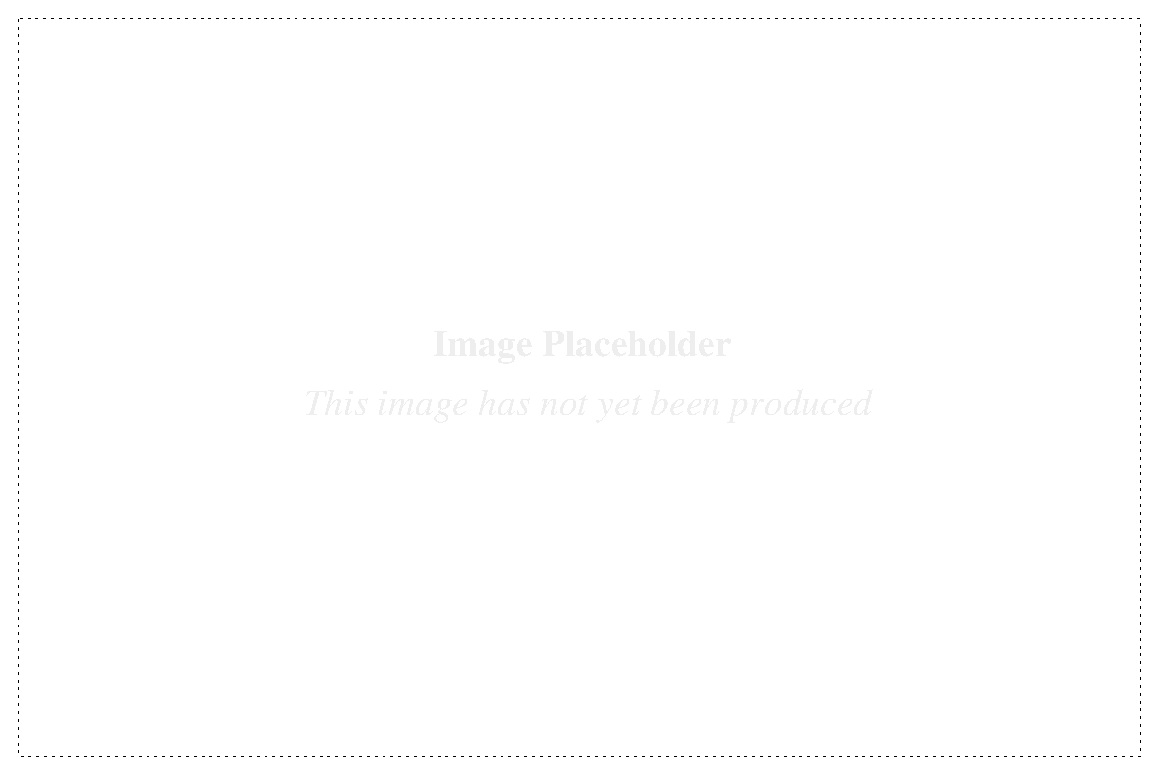
\includegraphics[width=8cm, height=4cm]{./eps/placeholder.eps}
%  \caption{Some single-column figure caption.}
%  \label{fig:myfigure1}
%\end{figurehere}
%
%\begin{figure*}[t]
%  \centering
%  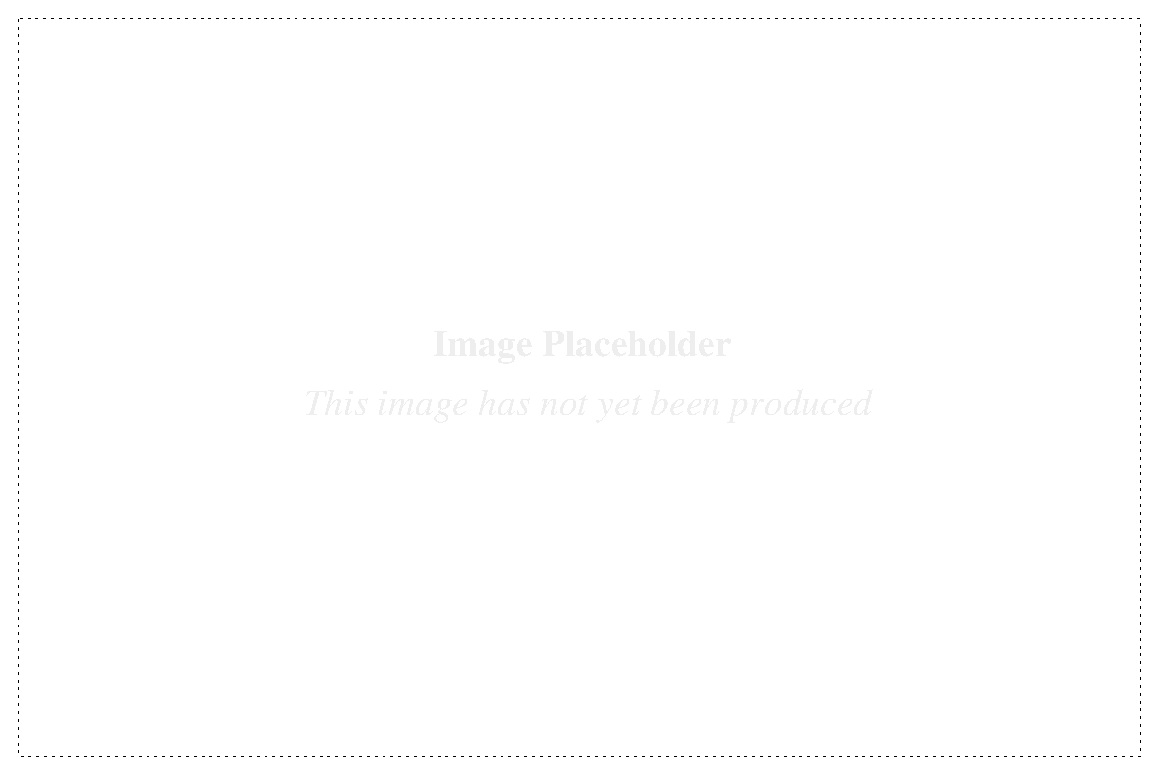
\includegraphics[width=16cm, height=4cm]{./eps/placeholder.eps}
%  \caption{Some wide-figure caption.}
%  \label{fig:myfigure2}
%\end{figure*}

\makeatletter
\newenvironment{tablehere}{\def\@captype{table}}{}
\newenvironment{figurehere}{\def\@captype{figure}\vspace{2ex}}{\vspace{2ex}}
\makeatother

%%%%%%%%%%%%%%%%%%%%%%%%%%%%%%%%%%%%%%%%%%%%%%%%%%%%%%%%%%%%%%%%%%%%%%%%%%%%%%
\begin{document}

\newcommand{\TODO}{\textbf{TODO\dots\ }}
\newcommand{\CITEME}{\textbf{[CITEME]}}
\newcommand{\INSFIG}{\textbf{Figure PLACEHOLDER}}
\renewcommand{\thefigure}{\arabic{figure}}
\newcommand{\citef}[1]{\textbf{Figure~\ref{#1}}}


\begin{mytitle}RATT	- Relatively Accurate TurnTable\end{mytitle}
\begin{mysubtitle}Relative turntable motion detection through mouse sensors\end{mysubtitle}
% Please do not insert a line here
\\
Zoppi Andrea\\
Matr. 765662, (andrea.zoppi@mail.polimi.it)\\
\begin{flushright}
\emph{Report for the master course of Embedded Systems}\\
\emph{Reviser: PhD. Patrick Bellasi (bellasi@elet.polimi.it)}
\end{flushright}

Received: <MONTH>, <DAY> 2012\\
\hspace{10ex}

\begin{myabstract} Abstract \end{myabstract}
Cheap jogwheel encoders for emulated DJ turntables are often inaccurate, due
to the low CPR in the order of some tens. Precise encoders are rather expensive
and are not convenient when detecting very fast rotations, because they become
too much accurate for the purpose.

The presented research tries to improve the detection of at least small and
slow relative rotations of the jogwheel, by employing a cheap COTS mouse sensor,
and keep the absolute position or fast rotation with the classic cheap optical
encoder.

A very crude HID demoboard was developed, so that some simple tests were done.
An extended proposal is also described, in order to achieve better performance
and more features, to match those of a commercial DJ controller.


\vspace{4ex}	% Please do not remove or reduce this space here.
\begin{multicols}{2}


%%%%%%%%%%%%%%%%%%%%%%%%%%%%%%%%%%%%%%%%%%%%%%%%%%%%%%%%%%%%%%%%%%%%%%%%%%%%%
\section{Introduction}
\label{sec:introduction}

In the latest years, the market of digital-DJ related products grew considerably.
By the way, cheap digtital turntable emulation is still tricky, because the
design of a cheap yet accurate jogwheel is still a challenge even with the
technology available today.

It is true that state-of-the-art processing units are very fast, but there are
still issues such as those related to protocol latency, precise and fast plate
motion detection, motion samples interpolation, and so on.

These issues are not a big problem for the average DJ, but they arise when
requiring a higher performance (e.g. \emph{scratch}) while keeping the costs
low.

The proposed approach is based on COTS components called \emph{optical motion/mouse
sensors}, which can provide a very good accuracy when detecting small local
motions, which is a behavior difficult to obtain with cheap encoders.

A simplified verison of the proposal was developed on a crude prototype, just
to check if it is worth at least for the average DJ -- the most demanding ones
do not care about the price of products, and still rely on timecoded vinyl
emulation even tough high CPR optical encoders are available at the same
overall price.


%%%%%%%%%%%%%%%%%%%%%%%%%%%%%%%%%%%%%%%%%%%%%%%%%%%%%%%%%%%%%%%%%%%%%%%%%%%%%
\section{Current market}
\label{sec:current_market}

The common commercial approaches can be divided into two groups: jogwheels
based on optical encoders, and reuse of vinyl turntables (or CD players) as if
they were digital jogwheels. These two technologies will be described in the
following, showing their pros and cons.

There exist also some other ways to emulate turntables, which are currently
still in a niche. For example, there are some touchscreen-based \cite{sm_emulator}
\cite{hn_touchosc} or capacitive \cite{stanton_scs3d} controllers, which
follow the market wave of touchscreen devices.
There are also some evolutions of the optical jogwheels, which are motorized
\cite{denon_sc3900} \cite{numark_v7} and thus more suitable for professionals,
but rather expensive.


%-----------------------------------------------------------------------------
\subsection{Optical encoder jogwheel controllers}

The most common technology for turntable emulation is based on optical encoders.
An optical encoder is a device which detects motion by counting the number of
steps an evenly-marked wheel performs. It is found in almost all purely digital
DJ \emph{controllers}, which in this context are referred to those remote
digital devices used by the DJ to control the user application. Some examples
of commercial controllers with jogwheels can be found in \cite{eks_op}
\cite{pioneer_ddjs1} \cite{vestax_vci400}.

Common jogwheels have a resolution (\emph{CPR, Counts Per Revolution}) in the
order of tens, thus are not suitable for \emph{scratching}, and are usually
addressed only in coarse track navigation, or \emph{bending}.
Even a resolution in the order of some hundreds cannot be enough for scratch
or precise motion tracking. For example, with a 720 CPR encoder it is possible
to detect only motions of half degrees, that for a 12 inches wide wheel is
still low -- keep in mind that a vinyl spins at roughly 150 degrees per second,
and good sampling should require at least 1500 samples per second to track it
decently enough.


\paragraph{System architecture}
The basic architecture of these controllers is shown is \citef{fig:hercules_mp3e2_schematic}.
The controller commonly has a set of input devices -- buttons, knobs,
sliders, \emph{etc.} -- so that the user can \emph{map}\footnote{
	Assign a triggered action to an input event
} these inputs to some software parameters, such as the play/stop events, or
the desired volume level.

A special kind of input device focused throughout this work is the optical
encoder, \TODO which will be described in depth later.

Commonly, there is a also set of output devices -- LEDs, displays -- so that
the user's sight should not always keep switching switched between the computer
monitor and the controller to see what is going on.

All these devices are managed by a MCU, which detects their changes, and
generates meaningful messages to be sent to the DJ software, or receives
messages from the latter.

The communication between the controller and the software is often performed
through an USB bus with HID/USB or MIDI/USB protocols, but some controllers
still rely on the plain old MIDI port (see Section~\ref{sec:controller_protocols}).

\begin{figurehere}
	\centering
	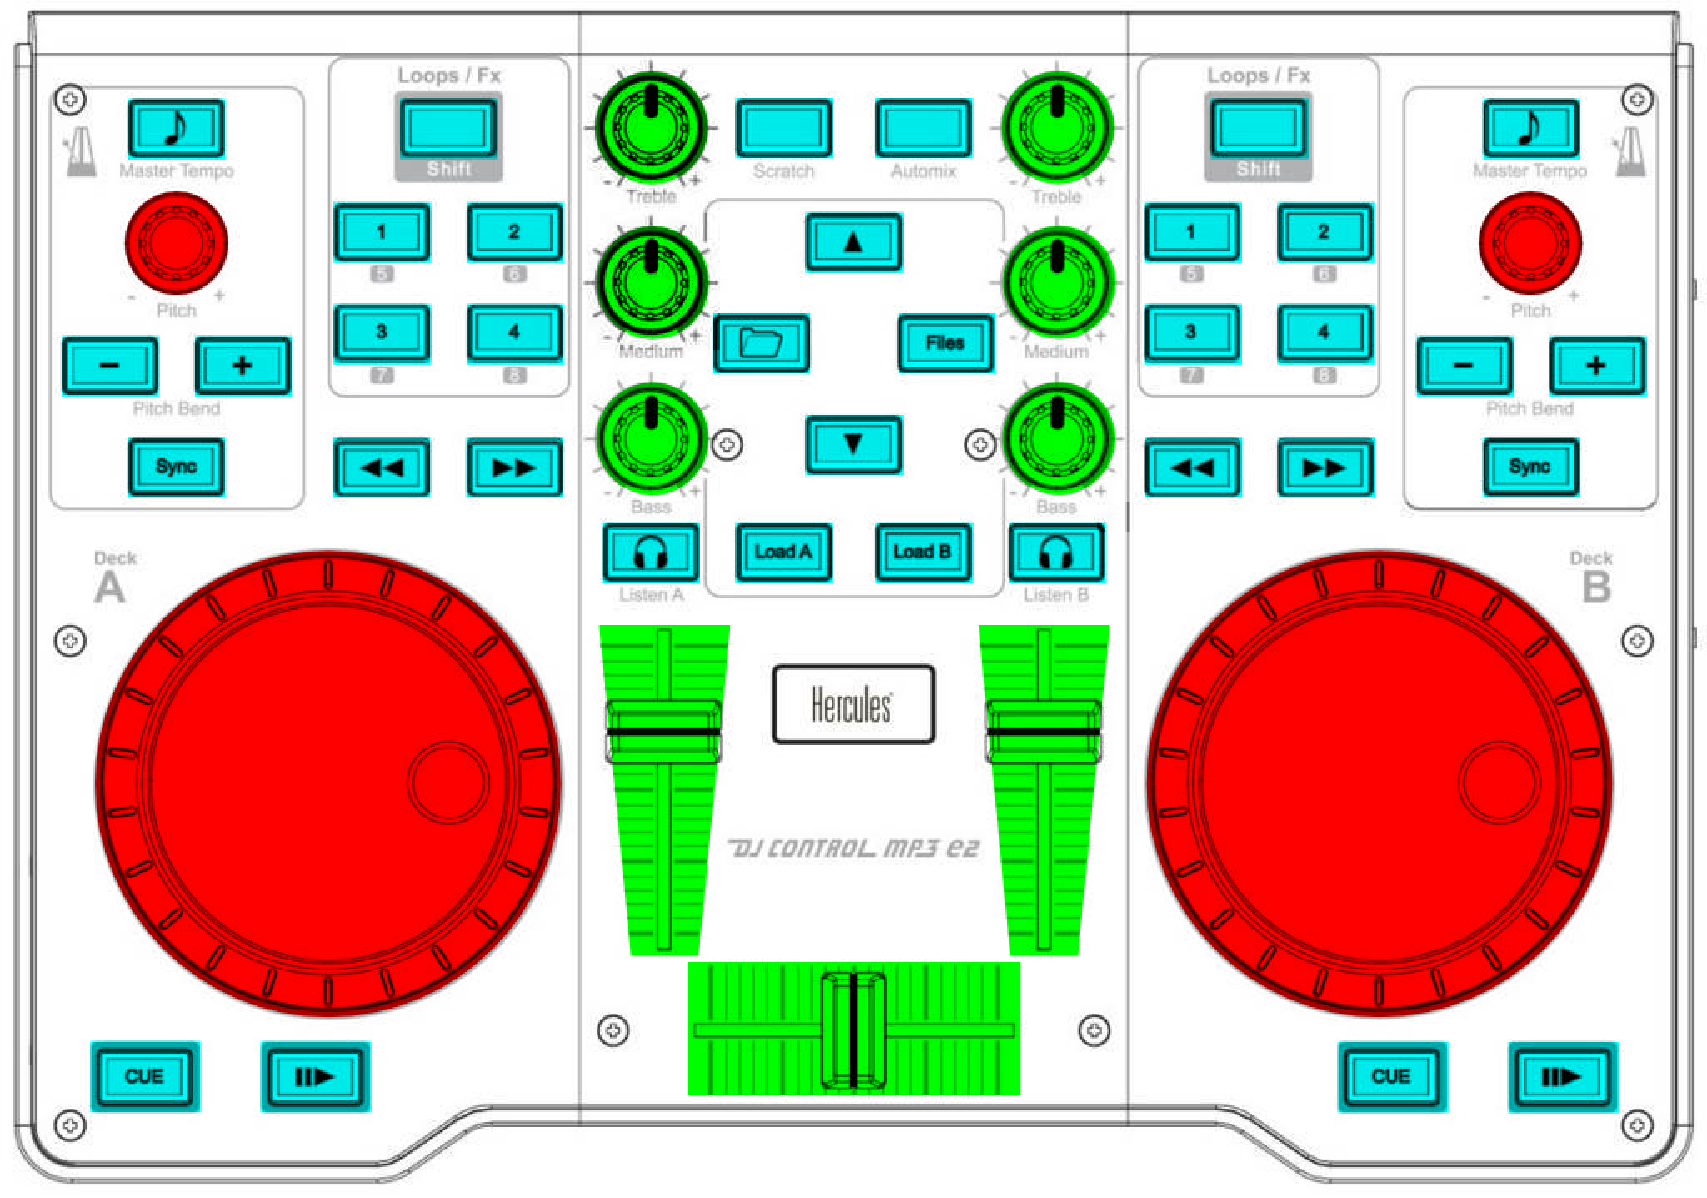
\includegraphics[keepaspectratio=true,width=\columnwidth]{images/hercules_mp3e2_schematic.pdf}
	\caption{\emph{Hercules DJ Control MP3 e2} \cite{hercules_djcmp3e2}
	intereface schematic with \textcolor{cyan}{buttons}, \textcolor{red}{incremental encoders},
	\textcolor{green}{sliders and knobs}}
	\label{fig:hercules_mp3e2_schematic}
\end{figurehere}


\paragraph{Wheel architecture}
The wheel is emulated with a so-called \emph{jogwheel}. It is a disc whose
full rotation is divided into equally-spaced angle slices. Each slice is
assigned a code.

Usually, the code is marked on the wheel with holes aligned on circles (see
\citef{fig:encoder_wheels}), so that holes can be detected by
light-detector sensors mounted on the chassis. The light-detector sensor is
almost always made with a LED which points towards the disc, and on the other
side the light is detected by a fast phototransistor. These light sensors are
positioned so that they can detect one and only one code per slice.

\begin{figurehere}
	\centering
	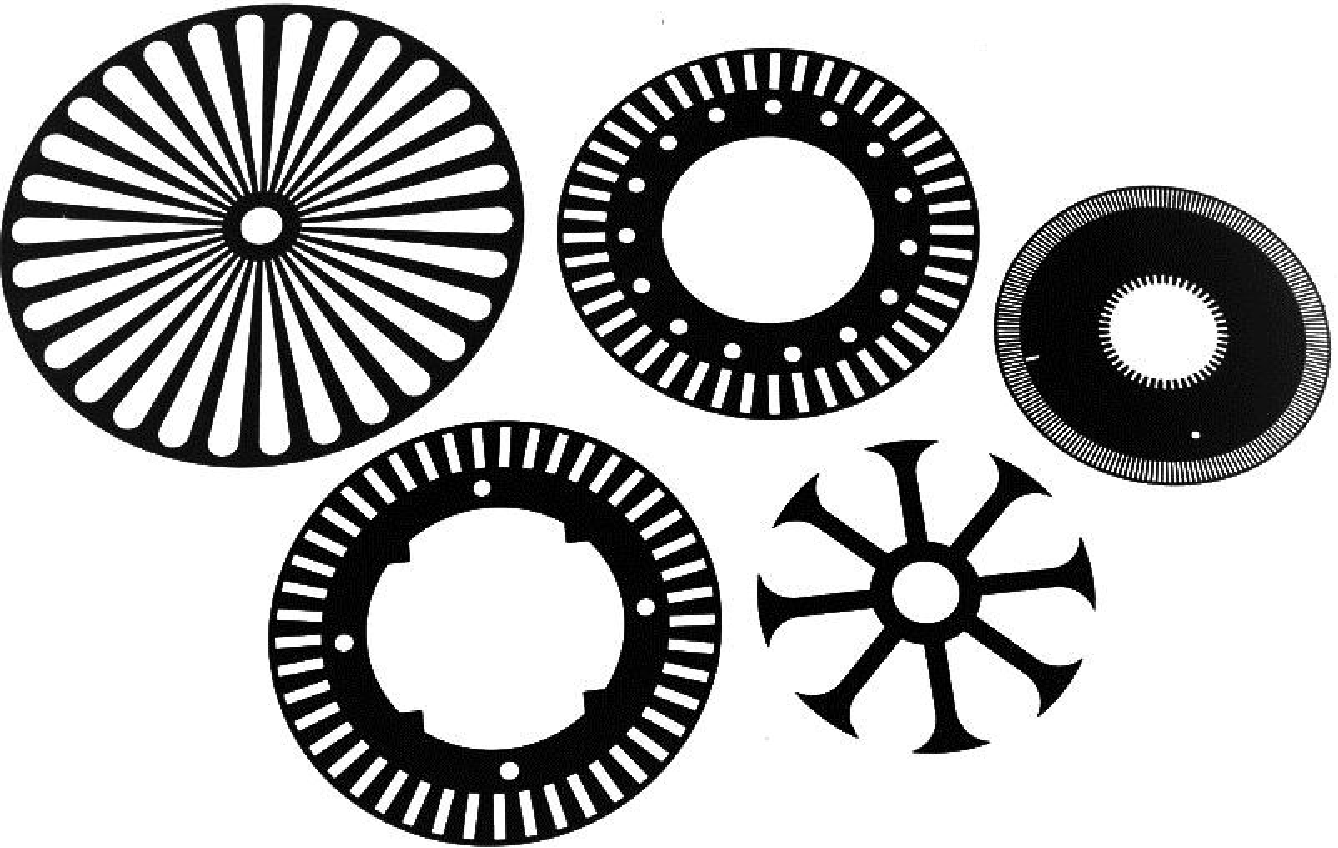
\includegraphics[keepaspectratio=true,width=0.9\columnwidth]{images/encoder_wheels.pdf}
	\caption{A set of incremental (quadrature) rotary encoder wheels}
	\label{fig:encoder_wheels}
\end{figurehere}

The code is either abolute or relative. Absolute encoders assign a unique code
to each slice, so that it is always possible to know the current wheel angle
by just reading the light-detector sensors outputs. Due to the need to have a
high number of bits, the number of holes can also grow exponentially (usually
as the power of two), and the production of precisely aligned marks and
sensors is expensive -- misaligned ones can provide misdetections of the
angle, even with robust codes such as the \emph{Gray code}.

Instead, relative encoders just need the two least significant bits of an
absolute code, thus cheaper to manufacture. On the other hand, it is not
possible to know the absolute rotation without any additional bits. This is
why there is often a mark which signals a full revolution been performed, and
needs an additional flag bit. The particular subset of the Grey code used for
the relative motion detection is called \emph{quadrature code}, because only 4
code sequences (phases) can be generated by moving to the adjacent wheel slice
as seen in \citef{fig:quad_wave}.

\begin{figurehere}
	\centering
	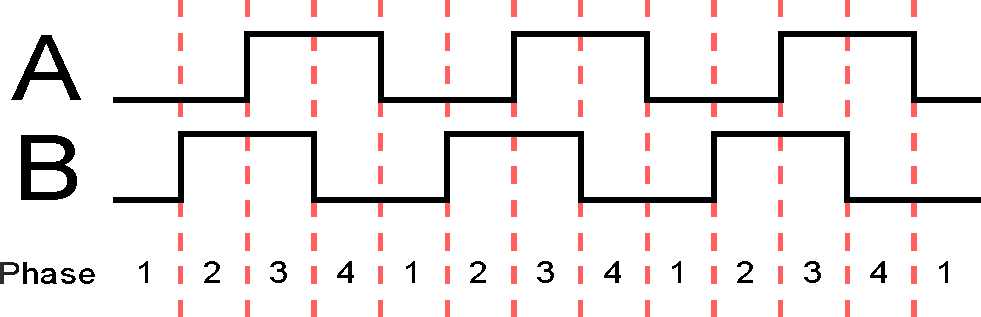
\includegraphics[keepaspectratio=true,width=0.9\columnwidth]{images/quad_wave.pdf}
	\caption{Quadrature pattern, going forward left-to-right}
	\label{fig:quad_wave}
\end{figurehere}

An example of jogwheel internals can be seen in \citef{fig:vestax_vci400_jogwheel}.
It is a close-up of the \emph{Vestax VCI-400} \cite{vestax_vci400} jogwheel
architecture, with a high-resolution wheel -- segments can be barely seen --
and an \emph{Agilent HEDS-9700} quadrature encoder.

\begin{figurehere}
	\centering
	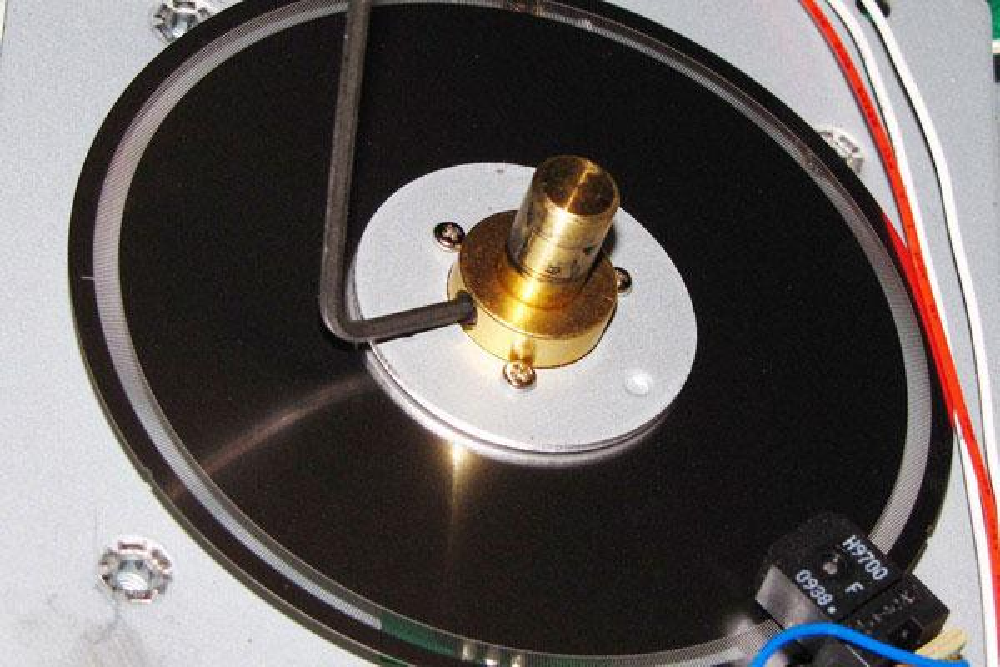
\includegraphics[keepaspectratio=true,width=0.8\columnwidth]{images/vestax_vci400_jogwheel.pdf}
	\caption{A \emph{Vestax VCI-400} jogwheel being disassembled}
	\label{fig:vestax_vci400_jogwheel}
\end{figurehere}


\paragraph{Motion detection}
When the user turns the wheel, the light-detector sensors can convert the
sight of light into the code assigned to the focused disc slice. The digital
code is then triggered by the MCU through some interrupts, and a message
containing the motion (or even the absolute angle) is sent to the user
software.

\paragraph{Pros}
\begin{itemize*}
	\item Easy to manufacture
	\item Code detection is inherently digital
	\item Fast code transitions can be processed easily
	\item A cheap MCU can handle jogwheels as well as all the other digital
		devices commonly found in DJ controllers
\end{itemize*}


\paragraph{Cons}
\begin{itemize*}
	\item Small motions have poor resolution with cheap encoders
	\item High resolution encoders are too much expensive for the purpose
\end{itemize*}


%-----------------------------------------------------------------------------
\subsection{Timecoded media turntable emulation}

An alternative way to emulate a turntable in software is to use a
\emph{timecoded audio track}, which is an audio stream coded so that the
software can read the track position just by decoding the incoming audio
stream.

This technique makes it possible to use existing turntables or CD players to
control the user software, which in turn will emulate the turntable behavior.

The good side of this approach is that a DJ, who already owns turntables or CD
players, can keep using them just by buying a sound card with the appropriate
audio inputs. This way the DJ can have almost perfectly the same old feeling,
because he is still using the same equipment.

On the bad side, vinyls and CDs are very sensible to usage, and decay easily.
This makes the timecode unreadable in the ruined parts of the support, where
software cannot always understand the code thus producing jittered or jerky
behavior.

In addition, turntable needles must follow tracks almost perfectly, or the
timecoded signal would degradate at the ADC side, especially the phase
component which is necessary for the purpose, but almost ignored in audio
players since the human ear has poor phase sensitivity.

Another bad point relates to the overall performance. It is true that with
this technique the performance is almost the same of a real vinyl, but the
need of an intermiate sound card, which in turn is often connected through the
USB bus, just makes low latencies hard to achieve, unless the host computer is
powerful and well optimised to reach soft-realtime requirements.

With a timecoded media is only possible to control the track position (phase)
and pitch (frequency), whihc is good for plain turntable emulation, but it is
impossible to use some features -- effects, precise loops, track preview, etc.
-- of some professional CD players.

When the disc spins at low speed, the intrinsic high-pass filter of needles
and soundcards will fade the signal, and it can become difficult to find the
zero-crossings while decoding (described further). This issue makes slow
scartches difficult to emulate because of jitter and corruption, and will be
mitigated with the work devolped in the rest of this document.

Finally, a novice DJ would hardly choose this approach, because the overall
price of the equipment can be rather high -- turntables/players + good
soundcard + accurate needles + cables + hi-performance computer can easily
exceed \$3000. 


\paragraph{System architecture}
A common commercial architecture \cite{rane_ssl} \cite{ni_tsp} can be seen in
\citef{fig:serato_setup}. The existing turntables or CD players are connected
to the appropriate soundcard inputs.

The soundcard can be placed either inside or outside the host computer.
Internal soundcards are very fast in transfering data from the incoming audio
signal to the CPU, thanks to the fast system bus (PCI or PCI-E).

However, as internal soundacards are almost always designed for desktop
computers but notebook computers are much easier to carry, the choice of an
external soundcard is the very most common.

External soundcards are mostly connected through an USB bus, but some
professional FireWire soundcards are still on the market. The USB bus has the
drawback of having a fixed minimum latency of 1~ms for isochronous signals,
which increases latencies even more, while FireWire is faster -- good internal
soundcards have a negligible latency.

\begin{figurehere}
	\centering
	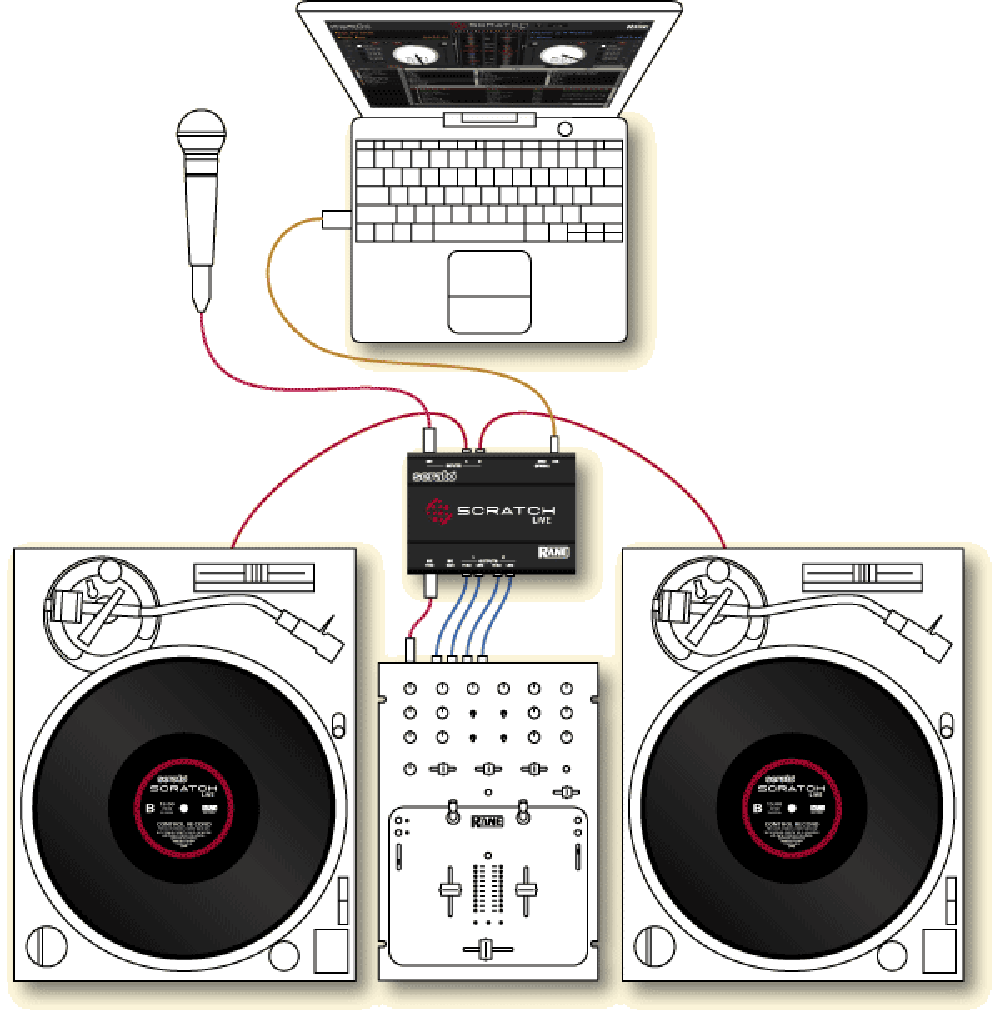
\includegraphics[keepaspectratio=true,width=0.9\columnwidth]{images/serato_setup.pdf}
	\caption{\emph{Serato Scratch Live} setup with two turntables}
	\label{fig:serato_setup}
\end{figurehere}


\paragraph{Signal pattern}
The timecoded signal is printed on the source media -- vinyl, CD -- with
patterns recognized by the specific user software. In general, the timecoded
signal is composed by a left sine and right cosine signals at a constant
frequency, usually in the range of 1~kHz to 3~kHz. The amplitude of each
half-wave of the same sign is slightly modulated with a proprietary digital
code, which represents the absolute position inside the whole timecoded track.

In \citef{fig:serato_timecode_slice} it is possible to see a slice of the
\emph{Serato Scratch Live} \cite{rane_ssl} timecode signal (aka
\emph{noisemap}), with some amplitude-modulated bits at the sine wave top
peaks.

\begin{figurehere}
	\centering
	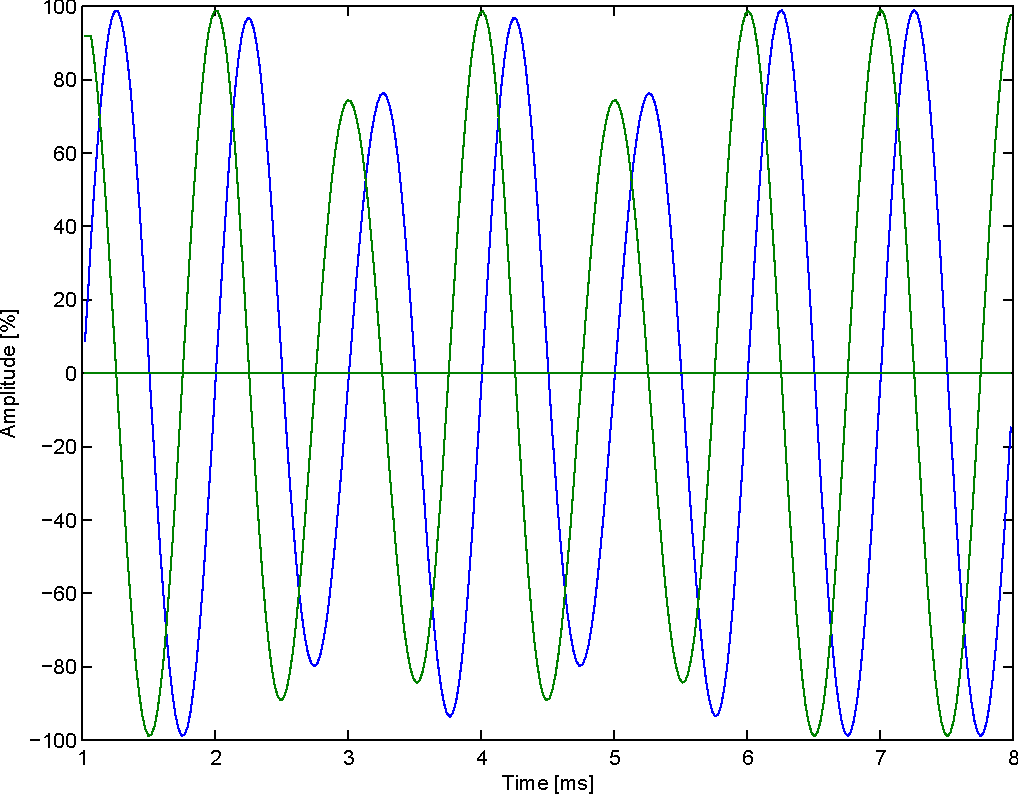
\includegraphics[keepaspectratio=true,width=\columnwidth]{images/serato_timecode_slice.pdf}
	\caption{Slice of the \emph{Serato Scratch Live} timecode}
	\label{fig:serato_timecode_slice}
\end{figurehere}

To read the code from a timecoded stream, it is sufficient to trigger a
positive-slope zero-crossing on one channel, and read the amplitude on the
other channel (peak), then convert the amplitude into a bit of the code
word. If the absolute position is not needed, instead of the whole code it
is possible to interpret the sine/cosine simply as a quadrature control
signal, for relative motions.

The code is designed to be decoded in both directions, so that the user can
navigate the emulated turntable just like a real vinyl. The most advanced
codes are designed to support fast error correction, because dust, decay of
the vinyl, or even EMF, would generate a corrupted signal.

In fact, if a single code is a bare label of the position, for example of 20
bits, it is necessary to read at least 20 consecutive half-waves. With a
nominal frequency of 1~kHz, the minimum latency would become 20~ms, which is
rather high for audio manipulation by a human. Advanced codes would still
correctly read the first 20 half-waves, but then each subsequent bit is
sufficient to get the adjacent code, with only 1~ms delay at 1~kHz.


\paragraph{Pros}
\begin{itemize*}
	\item Same old equipment
	\item Just add soundcard to a computer
	\item Natural feeling and performance
\end{itemize*}


\paragraph{Cons}
\begin{itemize*}
	\item Needs high quality components in the signal chain
	\item Expensive for a novice
	\item Signal subsceptible to corruption
	\item Bad tracking at low speeds
	\item Expensive signal processing
\end{itemize*}


%%%%%%%%%%%%%%%%%%%%%%%%%%%%%%%%%%%%%%%%%%%%%%%%%%%%%%%%%%%%%%%%%%%%%%%%%%%%%
\section{Simplified proposed approach}
\label{sec:simplified_approach}

The proposed approach was developed so that it is possible to achieve good
performance both at high and low speeds, without introducing expensive parts.

The main idea is to use a mouse sensor to measure slow local motions, which
are difficult to process with timecode, and need high resolution jogwheels.
As seen in the previous section, this is not possible with cheap designs.
Slow local motions are common when scratching or trying to reposition the
virtual needle of the emulated turntable, for example when the DJ is searching
for a good point where to start playing from (\emph{cue} point).

When the disc is spinning at cruise speed, or when the rotation is fast
enough, the classic methods can be used to keep track of the position.
Mouse sensors, in fact, are not able to keep track of absolute movements,
especially when they are very fast. Anyway, even cheap sensors have a
resolution in the order of several hundreds, if not thousands, DPIs nowadays.
As proven later, the disc can theoretically be divided in thousands slices,
thus providing a local resolution higher than the most expensive encoders on
the market -- obviously in the set of those affordable for a DJ, not the
state-of-the-art encoders for hi-end industrial machineries.

In the following, a simplified prototype will be presented. A low-end MCU and
a standard COTS mouse sensor were chosen, just to see if it is possible to
achieve good performance with a simple circuit. Unfortunately, the performance
was not that good, mainly because of latencies in both the MCU and the sensor.
This is why an advanced approach will be proposed in the next section, which
should provide a much better response and could handle more peripherals then
the only wheel.


%-----------------------------------------------------------------------------
\subsection{Hardware architecture}

The simplified prototype has a very crude hardware architecture. It is split
into three modules: the \emph{controller board} (aka \emph{main board}), the
\emph{sensor board} and an optional \emph{timecode preamp board} for the use
with timecode media. This subdivision was done just to decouple the controller
with the sensor, for further experiments with other hardware configurations.


\paragraph{Controller board}
The controller board in \citef{fig:board_photo} hosts the MCU, a
\emph{PIC18LF14K50} \cite{microchip_pic18lf14k50} by \emph{Microchip}, which
is a 8-bits MCU running at 48~MHz (16 MIPS). It is fast enough to handle a
single wheel, but nothing more advanced such as DSP, which is left to the
user software application.

This board also mounts the voltage regulator, to get 3.3~V from the standard
5~V provided by the USB host. Bulk capacitors keep it stable.

There are also a user button for input, and three LEDs for user interactions.

A standard UART can be used for basic messaging with an optional text console.

There are also two pins dedicated for an additional quadrature encoder input.
They can be configured to be directly coupled with the MCU comparator
interrupts, in order to trigger encoder changes.

Finally, to communicate with the sensor module some control and interrupt
signals, and a half-duplex serial port are provided.

\begin{figurehere}
	\centering
	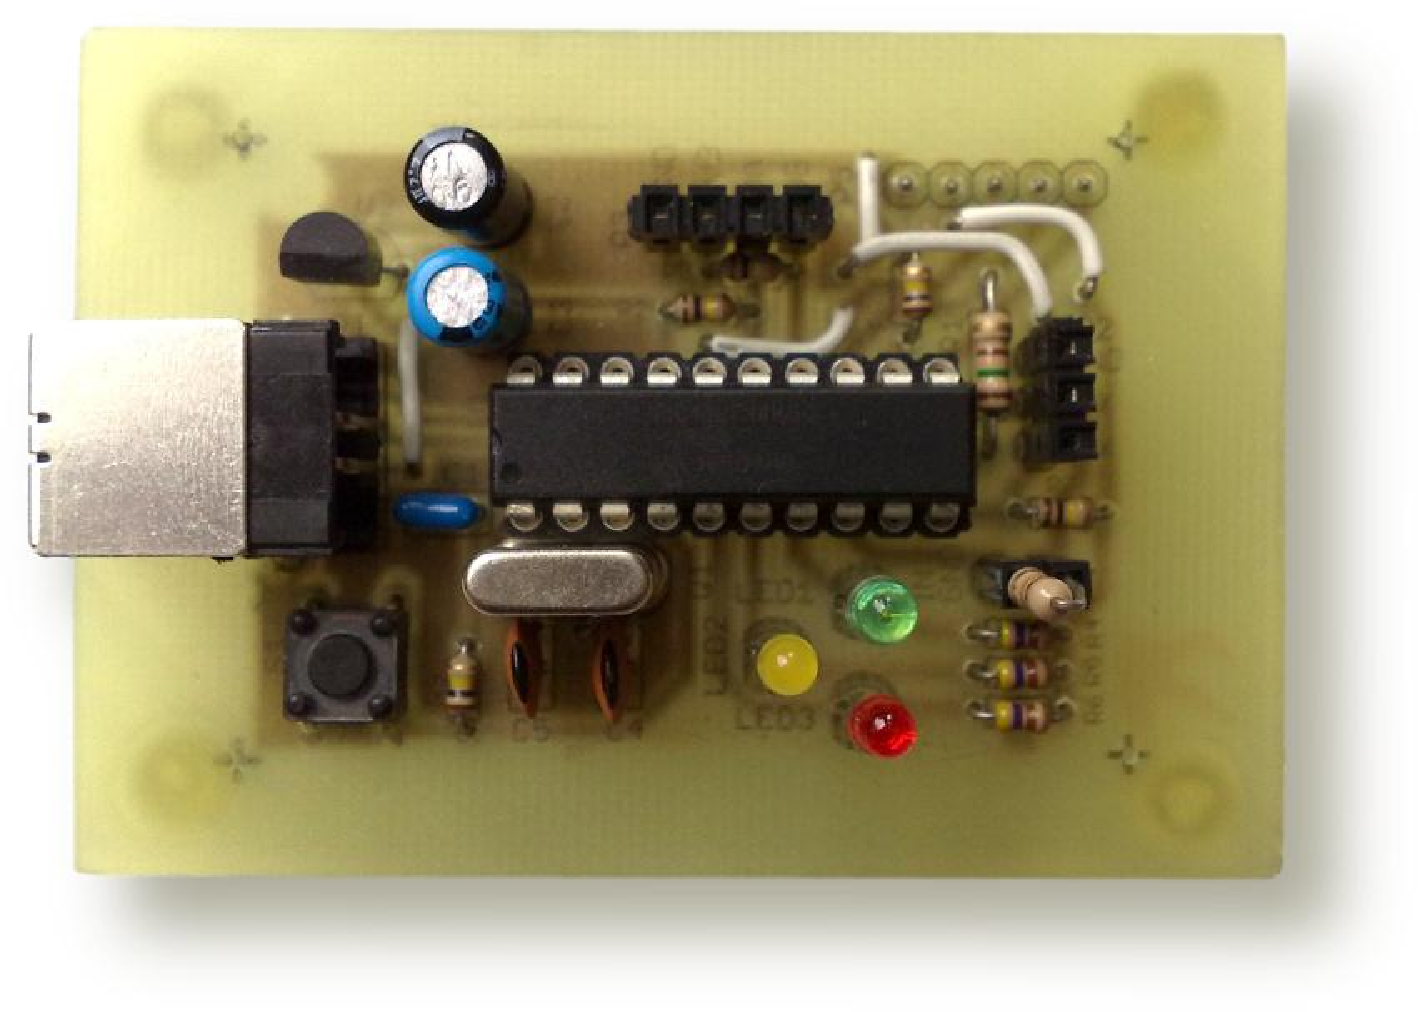
\includegraphics[keepaspectratio=true,width=\columnwidth]{images/board_photo.pdf}
	\caption{The controller prototype board}
	\label{fig:board_photo}
\end{figurehere}


\paragraph{Sensor board}
The sensor board in \citef{fig:sensor_photo} simply hosts the mouse sensor,
the surface illumination LED, and the lens. The sensor is an \emph{ADNS-2080}
\cite{avago_adns2080} by \emph{Avago}. It is a sensor aimed at office users,
with average performance and low cost. As for the MCU, higher performance
modules are on the market, but the challenge of this proposal was to find a
basic average solution, which can be improved with further research. Briefly,
the sensor can reach an interesting resolution of up to 2000~DPI, and motion
speed up to 30~in/s (76.2~cm/s). There is no guarantee of minimum or maximum
latencies, because the clock speed is variable.

\begin{figurehere}
	\centering
	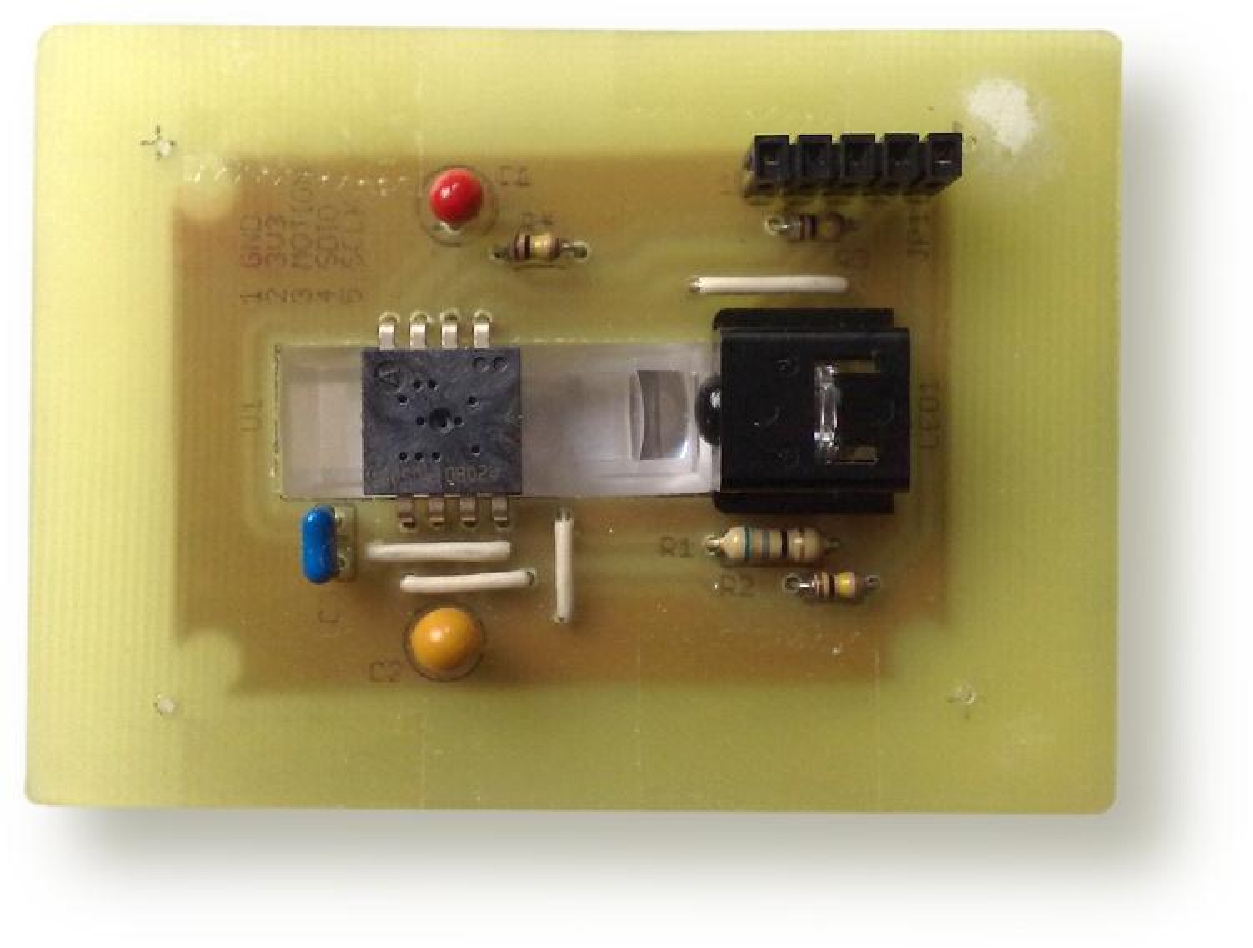
\includegraphics[keepaspectratio=true,width=\columnwidth]{images/sensor_photo.pdf}
	\caption{The optical motion sensor prototype board}
	\label{fig:sensor_photo}
\end{figurehere}


\paragraph{Timecode preamp board}
An optional board, seen in \citef{fig:preamp_photo}, was designed to properly
amplify a \emph{Line} -- no \emph{Phono}! -- timecode signal so that it can be
recognized by comparators of the controller board.

Each audio channel can be amplified in amplitude, by controlling the inverting
gain of the opamp with a potentiometer. A spare opamp generates the $V_{DD}/2$
voltage reference for single-supply conditioning.

Two LEDs help the user in keeping the overall timecode level compatible with
the comparator inputs on the controller board, by warning if the signal is
near saturation, or too low to be squared correctly by comparators.
In fact, when the volume is too low or saturates, the sinusoidal timecode
signals won't be squared with 50\% duty cycle, which can generate some jitter.

\begin{figurehere}
	\centering
	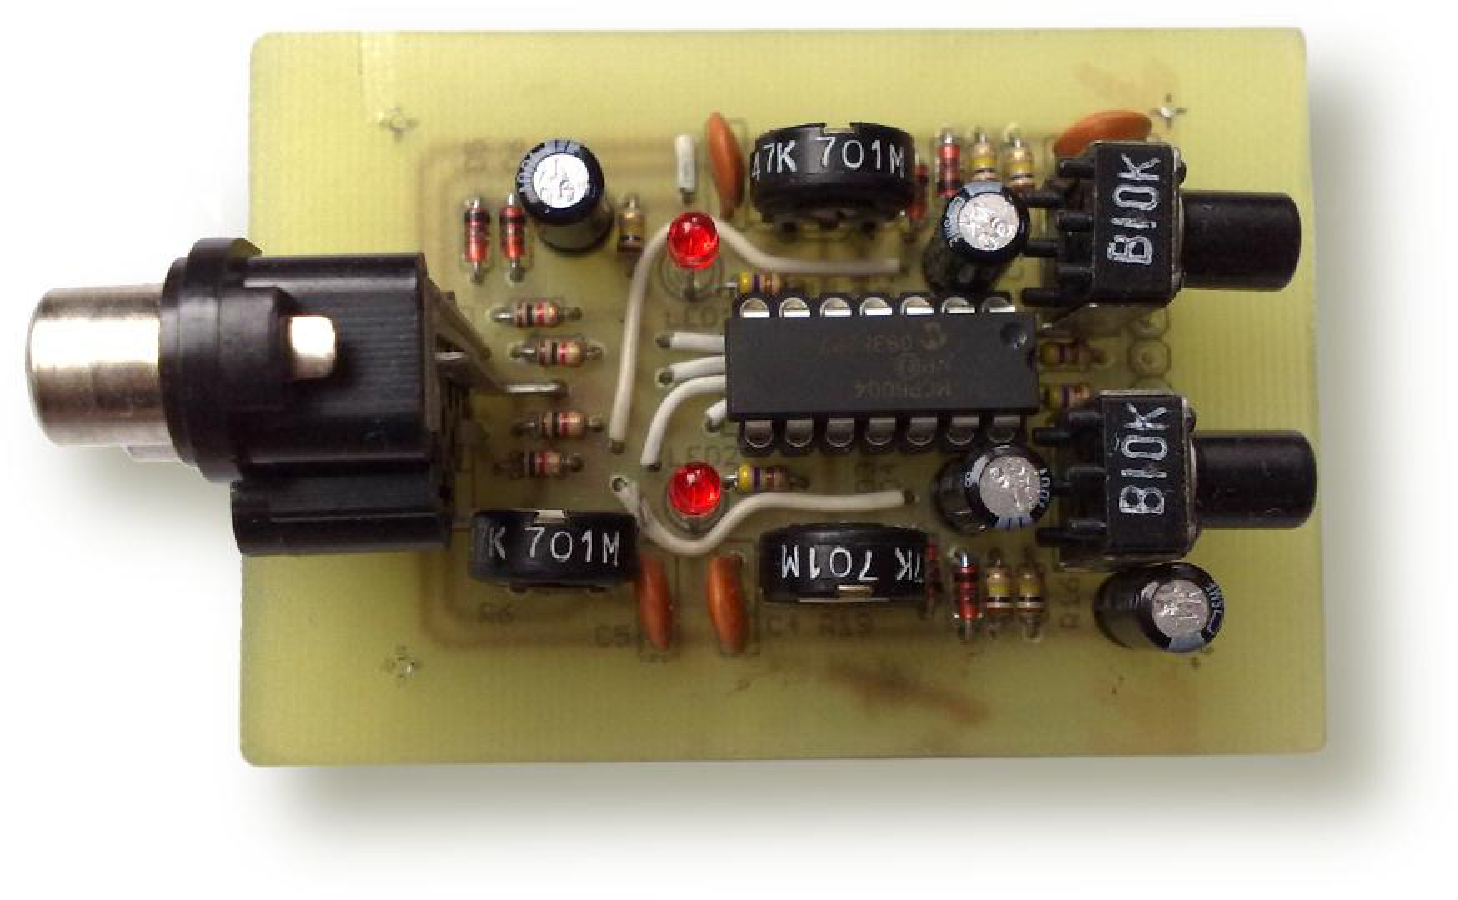
\includegraphics[keepaspectratio=true,width=\columnwidth]{images/preamp_photo.pdf}
	\caption{The timecode preamplifier prototype board}
	\label{fig:preamp_photo}
\end{figurehere}


%-----------------------------------------------------------------------------
\subsection{Firmware architecture}

Due to the lack of a \emph{Real-Time Operating System} (\emph{RTOS}) support
on the chosen MCU, the application was written in a \emph{while-loop} fashion,
with \emph{interrupt-driven} tasks at \emph{high priority}.


\paragraph{Bootloader}
In order to simplify firmware deployment, a HID bootloader was added to the
development prototype. This will occupy the first 2048 words of the program
space, which is not that small. The bootloader is the one provided by the
\emph{Microchip Application Libraries} \cite{microchip_mal}, and implements
HID control.

The bootloader can be called by plugging RATT into the USB host socket, while
pressing the user button. The developer can then use the HID bootloader
software provided by Microchip to download the complied HEX executable to the
program memory of the MCU.


\paragraph{HID/USB module}
\TODO


\paragraph{LED module}
The LED module simply drives the three LEDs on and off.


\paragraph{Encoder module}
A small software module (\emph{incenc}) decodes the quadrature signal fed by a
rotary encoder, or exploited from a properly timecoded media stream.

The quadrature encoder waves are gathered by the MCU by triggering interrupts
in a rather tricky way. The two quadrature inputs, namely \emph{A} and
\emph{B}, are connected to the negative inputs of the two comparators of the
chosen MCU. The comparators have an internal reference (positive input)
voltage fed by the internal DAC module at $V_{DD}/2$, with a small hysteresis.

Whenever the quadrature signal (A or B) crosses the reference voltage, an
high-priority interrupt is generated. The ISR detects the current quadrature
phase and accumulates the single step into a global delta counter.

The delta counter can then be collected by the (slower) HID report generator,
which resets it.

The initialization routine simply configures the voltage reference DAC, the
two comparators, and interrupts.

There is no background service, since all the processing is triggered by
interrupt events.


\paragraph{Sensor module}
Another software module (\emph{adns2080}) handles the mouse sensor. This
module provides communication rountines over the SPI port of the MCU in a
half-duplex fashion.

All the communication routines are blocking, but this is not a problem because
they are executed in the background service (main loop) of the firmware
architecture.

An initialization routine configures the SPI port, then the mouse sensor. Its
setup will allow for top-performance (no low-power states), 12-bits deltas
reporting, and active-low level-sensitive motion interrupt generation.
This routine will also check for proper communication with the daughter board.

The high-priority motion interrupt is generated by the sensor whenever motion
is detected. This interrupt is cached by raising a firmware flag. The high
priority level will minimize CPU cycles for this very simply operation.

The background service polls for the interrupt flag, and starts a \emph{motion
burst} read, which collects motion deltas over the serial port by minimizing
dead times. Deltas are accumulated on global counters, which will be gathered
by the HID report generator and thuse reset.


\paragraph{Main module}
The main module, also called the \emph{app}, initializes the system, handles
the main loop, and provides some interrupt functions.

The initialization sequence calls the initialization of all the sub-modules.

The main loop cycles through the \emph{service task} of the sub-modules, so
that motion deltas are computed for both the sensor and incremental encoder
modules. If the deltas are meaningful and the HID transmission endpoint is
available, a new HID report is built and sent to the host.

The two interrupt handlers, one for high-priority and one for low-priority
interrupts, will obviously handle events generated by peripherals.

Some functions are dedicated to locking and unlocking of the application
resources, and are basically wrappers respectively to global interrupt disable
and enable.


\paragraph{Tasks organization}
The modules are organized in a \emph{while-loop} fashion, because the chosen
MCU has not enough computational power, nor a stack manageable by an actual
RTOS.

An initialization procedure will turn all the modules on, and enables
interrupts. After that, the main loop is entered.

Inside the main loop, incremental encoder and mouse sensor deltas are gathered
and, if the USB endpoint is free, sent by an HID report.

Fast and simple interrupt events are processed by the high-priority ISR, while
communication events, which are slower, are processed by the low-priority ISR.


\paragraph{Remarks}
\TODO


%-----------------------------------------------------------------------------
\subsection{Software architecture}

\TODO


\paragraph{HID/USB connectivity}
\TODO


\paragraph{Device description}
\TODO


\paragraph{Device mapping}
\TODO


%-----------------------------------------------------------------------------
\subsection{Sizing and computations}

\TODO


%-----------------------------------------------------------------------------
\subsection{Field results}

\TODO


%%%%%%%%%%%%%%%%%%%%%%%%%%%%%%%%%%%%%%%%%%%%%%%%%%%%%%%%%%%%%%%%%%%%%%%%%%%%%
\section{Advanced proposed approach}
\label{sec:advanced_approach}

Due to the few capabilities of the simplified approach, which is just for
basic research and demonstration purposes, a more advanced way to achieve
better results is presented in the following. No prototype was made, but a
high-level description of the target architecture can drive the development
of an actual device.

Basically, the advanced approach exploits the computational power of the most
recent MCUs in order to provide faster motion detection and processing rate,
as well as the opportunity to handle tasks outside those for the motion
detection.

\TODO


%-----------------------------------------------------------------------------
\subsection{Hardware architecture}

The generic architecture reflects that of complex digital DJ controllers
which offer jogwheels (often touch-sensitive), but also buttons, knobs,
sliders, lights, displays, external connections, audio piping to DSP, and so
on.

By choosing a fully-featured MCU of nowadays, such as the \emph{STM32~F4}
family, it is possible to handle almost all these devices with only one MCU,
at reduced overall price. Obviously, some additional chips are still needed
-- motion sensors \emph{in primis} -- but the whole architecture can be shrunk
into a few chips.


\paragraph{Digital inputs}
The most basic type of inputs is \emph{discrete-state} (\emph{digital)} input
devices, such as buttons, switches, toggles, and so on. In order to handle
them, a \emph{matrix} topology often suffices, such as the one seen in
\citef{fig:keypad}. Such matrix can be scanned row-by-row through row
(de)multiplexing, and then processed by the \emph{digital inputs task} of the
firmware \CITEME.

\begin{figurehere}
	\centering
	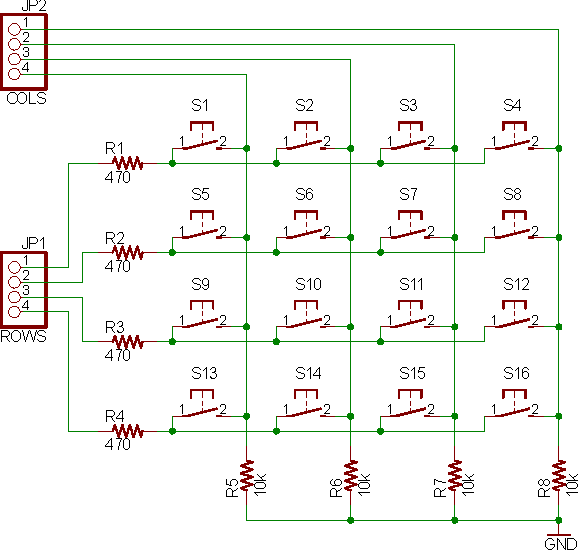
\includegraphics[keepaspectratio=true,width=0.8\columnwidth]{images/keypad.pdf}
	\caption{A $ 4 \times 4 $ matrix keypad driven by an 8-bits port}
	\label{fig:keypad}
\end{figurehere}


\paragraph{Analog inputs}
The user should also be able to control DJ software parameters with a 
continuous values range. Such values are provided through knobs and sliders.
Electrically, these devices are all potentiometers connected to the ADC module
of the MCU through its analog multiplexer, as shown in \citef{fig:pots_mcu}.
The analog values will then be converted by the ADC and processed by the
\emph{analog inputs task} of the firmware \CITEME.

\begin{figurehere}
	\centering
	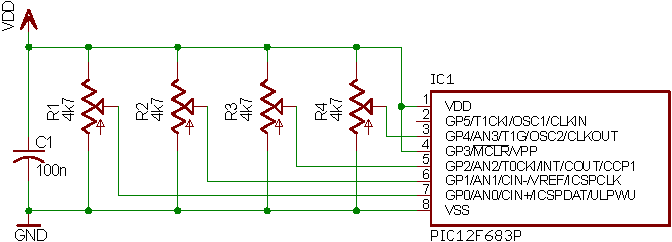
\includegraphics[keepaspectratio=true,width=\columnwidth]{images/pots_mcu.pdf}
	\caption{4 potentiometers connected to a MCU, through its built-in analog
	MUX and ADC}
	\label{fig:pots_mcu}
\end{figurehere}


\paragraph{Jogwheels}
Jogwheels are fundamentally those developed in the simplified approach at
Section~\ref{sec:simplified_approach}. Each jogwheel is made by a
medium-resolution optical quadrature wheel and its encoder, plus an optical
motion sensor.

The quadrature encoder, thanks to its fairly low speed, can be handled by
MCU interrupt signals (edge-triggered, both signs).

Instead, motion sensors must be connected to the appropriate digital bus
(I2C, SSP, SPI), and additional pins to suitable inputs.

Jogwheels should also provide touch-sensitivity, so that a digital signal
(see above) can be generated when the user puts fingers on the wheel.
There are different ways to provide touch sensitivity, but will not be
covered in this document.


\paragraph{Lights}
Some light can help the user in keeping track of some DJ software states.
Thanks to their very low current consumption and simplicity, LEDs are
always the best choice.

Simple lights can be driven directly by the MCU digital pins, in
any desirable fashion -- could it be direct coupling, LED matrix,
or charlieplexing. These lights can be either on or off.

Dimmed lights are more complex to handle, and need to be connected to PWM
outputs to give an intensity effect to the human eye, proportional to the
PWM duty cycle. Due to scarcity of such outputs, this feature is often not
implemented at all, or applied to simple behaviors -- for example, the
\emph{M-Audio Torq Xponent} \cite{maudio_xponent} gives the so-called
\emph{Christmas tree} effect, with all LEDs beign modulated by the music tempo.


\paragraph{Displays}
Very advanced controllers sometimes provide information through one or more
displays. There are so many display types on the market, that it is difficult
to suggest one. Anyway, for pure text displays, or generally soft-realtime
information visualization, the connection to one among the common UART, I2C,
SPI buses is enough.

\TODO


%-----------------------------------------------------------------------------
\subsection{Firmware architecture}

\TODO


\paragraph{Main module}
\TODO


\paragraph{HID/USB module}
\TODO


\paragraph{LED module}
\TODO


\paragraph{Encoder module}
\TODO


\paragraph{Sensor module}
\TODO


\paragraph{Debug module}
\TODO


\paragraph{Tasks organization}
\TODO


\paragraph{Remarks}
\TODO


%%%%%%%%%%%%%%%%%%%%%%%%%%%%%%%%%%%%%%%%%%%%%%%%%%%%%%%%%%%%%%%%%%%%%%%%%%%%%
\section{Appendix A - Optical motion (mouse) sensors}
\label{sec:mouse_sensors}

Optical motion sensors are commonly found in computer pointing devices called
\emph{mouses}. The job of such sensors is to capture a \emph{photograph}
(i.e. a \emph{frame}) of what is beneath, compare it with the previous one,
and finally compute the motion (i.e. the distance) from the previous relative
position.

Their main strength is the achievement of very high resolution comparisons, in
the order of hundreds, if not thousands, \emph{Dots Per Inch} (\emph{DPI}), at
a very low price -- less than a dollar for average sensors, or a few dollars
for high performance (\emph{gaming}) mouse sensors. Also, the maximum
detectable speed is in the order of some tens inches per second, compatible
with human and motion.

As a drawback, the absolute accuracy is poor, as they are designed to capture
the slow relative movements of a screen cursor. It can be repositioned by
the software, or its relative motion is exploited for some games (e.g.
\emph{First Person Shooters}), thus making absolute motion tracking clueless.

As can be inferred from the previous statements, mouse sensors come in
different classes, based on their main applications. The most common sensors
are for office or home use, and provide average accuracy and speed. Other
sensors are designed for wireless devices, and can provide automatic switching
between average (or high) and low performance, based on the amount of
interaction of the user in the last time window. The most advanced sensors are
for those professionals or enthusiasts who need very high speed and precise
motion detection, for example for pro-gamers.


%-----------------------------------------------------------------------------
\subsection{Architecture and operation}

A generic mouse sensor is composed by components of various nature, as seen
in \citef{fig:sensor_assembly}.

\begin{figurehere}
	\centering
	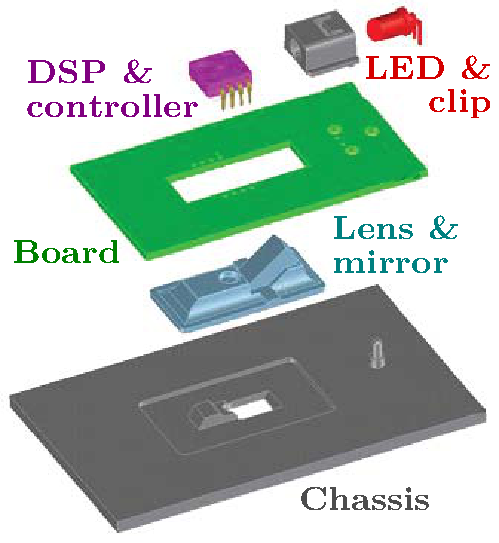
\includegraphics[keepaspectratio=true,height=5cm]{images/sensor_assembly.pdf}
	\caption{Common motion sensor assembly}
	\label{fig:sensor_assembly}
\end{figurehere}


\paragraph{Light source}
A light source, typically a LED, or a laser for the most advanced models,
illuminates the small surface to be captured.


\paragraph{Lens}
A lens focuses the surface to get the best resolution at detector side.
The lens also increases the effectiveness of the light source on the surface,
when correctly focused on the surface beneath through a mirror.

Usually the lens is placed at a few millimiters from the surface, and
it is quite important to keep the nominal distance for the best perofrmance.


\paragraph{CCD}
The actual light sensor is a common \emph{Charge-Coupled Device}
(\emph{CCD}). It is designed to be very fast, to achieve a high frame rate.
It is also sensitive to a very small light spectrum, e.g. the infrared one,
so that environmental light noise is rejected, and image artifacts are acquired
better.

There are also some considerations based on the light type. LED-based devices
work well with all the bumpy surfaces, even the dark ones, but cannot work
on trasparent ones, where the reflection is very bad. They are suited for
everyday use.
Instead, laser-based give a way better tracking on all surfaces but the dark
ones. The tracking performance is suited for professionals.


\paragraph{DSP}
The frame impressed on the CCD is then processed by an \emph{ad-hoc}
\emph{DSP}, which computes the distance -- in $(x,y)$ frame coordinates --
from the previously acquired frame. The DSP must be fast enough to reach the
10x-in/s maximum detected velocity in both directions.


\paragraph{Controller}
Finally, the controller accumulates the DSP deltas. Some configuration
parameters and device properties, along with deltas, can be accessed through
an interface to an external controller.


%-----------------------------------------------------------------------------
\subsection{Communication}

Optical motion sensors communicate with an external processor through an
interface which often belongs to standard I/F types, even though some pins
are frequently added for faster or ad-hoc operation -- chip shutdown, chip
selection, flow control, and so on.


\paragraph{Quadrature}
Sensors with only quadrature wave outputs (see \citef{fig:quad_wave}) are now
outdated, because they do not offer any advanced features, and require an
interrupt-driven counter at controller side. On the other hand, quadrature
outputs can be used with any device which natively accepts such signals.


\paragraph{I2C}
When requiring some more flexibility, an I2C bus is already enough for average
sensors. Due to its message-based nature, it is possible not only to read
internal counters, but also to get and set come configuration parameters.

On the other hand, the I2C protocol introduces some unnecessary latencies
due to handshaking and baud rate -- standard I2C is only at 100~kb/s, fast
mode at 400~kb/s.

\INSFIG


\paragraph{SSP/SPI}
When requiring slightly higher speed and lower latency, it is possible to
adopt \emph{Synchronous Serial Port} in both \emph{Serial Peripheral Interface}
(\emph{SPI}) or \emph{3-wire}, respectively with full-duplex and half-duplex
capabilites, to communicate with motion sensors.

They usually do not require handshaking, even though some control pins are
often used in such a way (e.g. the common \emph{shutdown} pin).
Also, the bit rate is often higher -- from 1~MHz to some tens -- even though
pratically not much higher than I2C.

An example of \emph{write} operation over a 3-wire SSP is shown in
\citef{fig:ssp_write}. The master device signals an incoming \emph{write}
operation, tells the register address and its value.

An example of \emph{read} operation over the same hardware is shown in
\citef{fig:ssp_read}. The master signals an incoming \emph{read} operation
and tells the address. After that, it lets the slave drive the SDIO line,
then eventually reads the addressed register value.

\begin{figure*}[t]
	\centering
	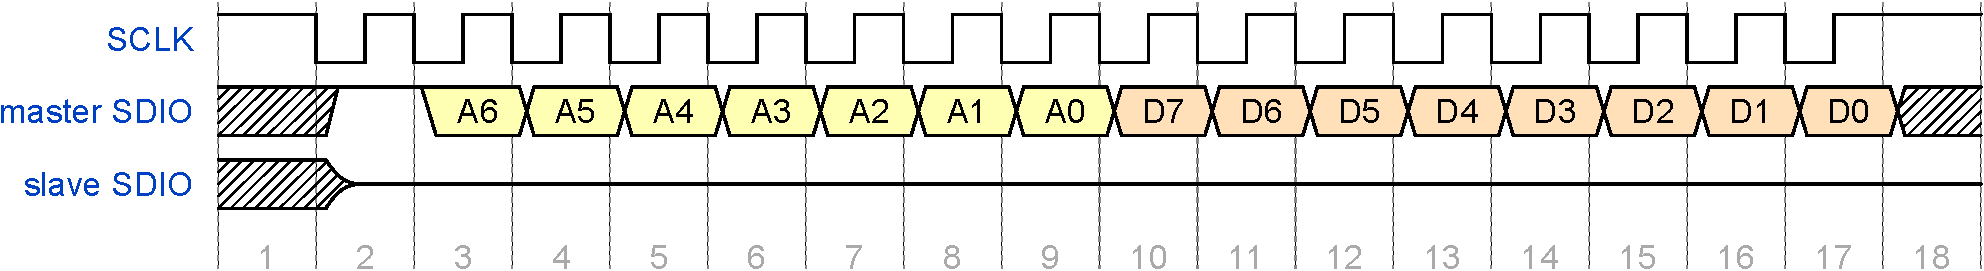
\includegraphics[keepaspectratio=true,height=1.8cm]{images/ssp_write.pdf}
	\caption{A write operation through an half-duplex, 3-wire SSP}
	\label{fig:ssp_write}
\end{figure*}

\begin{figure*}[t]
	\centering
	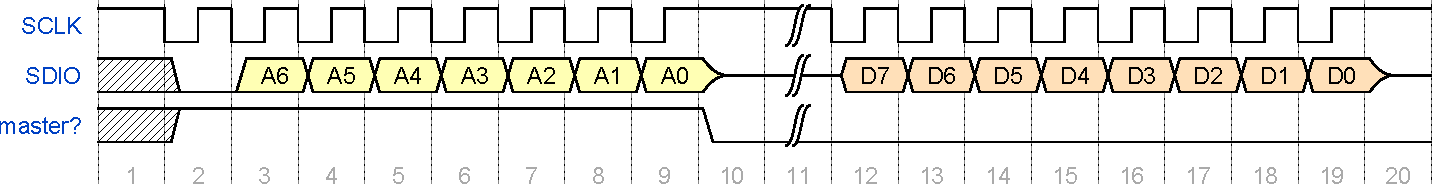
\includegraphics[keepaspectratio=true,height=1.8cm]{images/ssp_read.pdf}
	\caption{A read operation through an half-duplex, 3-wire SSP}
	\label{fig:ssp_read}
\end{figure*}


%%%%%%%%%%%%%%%%%%%%%%%%%%%%%%%%%%%%%%%%%%%%%%%%%%%%%%%%%%%%%%%%%%%%%%%%%%%%%
\section{Appendix B - Controller communication protocol comparison}
\label{sec:controller_protocols}

When developing a music-oriented controller, there is always a debate on which
communication standard is most suitable for the application. The most common
standard are described in the following.


%-----------------------------------------------------------------------------
\subsection{Plain MIDI}

The truly \emph{de-facto} standard in music-oriented communication is the
\emph{Musical Instrument Digital Interface} (\emph{MIDI}). This was
developed in the '80s to be easy and cheap to manufacture, robust and rather
complete for standard music production, with some degree of freedom for
sub-protocols developed by manufacturers. It is still widely supported by
nowadays digital music equipment.

Common output and input circuits can be seen respectively in \citef{fig:midi_out}
and \citef{fig:midi_in}. Basically, it is a standard serial point-to-point
connection based on common UARTs. Data transmitted by the UART is converted
into current bursts, which light the optocoupler at the receiver. The
optocoupler provides galvanic isolation, so that no \emph{current loops} can
create audible noise in the target device, which used to be a synthesizer in
the first place.

Each MIDI connection can handle up to 16 \emph{channels}, i.e. virtual music
devices. This is enough for common synthesizers, but not to drive an entire
production studio.

The event-based nature of the protocol makes it suitable for most of the
situations, but for events which could be accumulated, or state streaming.
For example, jogwheels could generate way too many motion delta events, usually
as Control Change messages, which would easily flood the entire bus. A packed
streaming state would be better suited in such cases.
Also, when transmitting to a host computer, its operating system (often
time-shared), software buffers can saturate while processing too many events
at a time, or complex sound textures.

The protocol does not support any kind of flow control. Massages can be lost,
partially received (ignored), contain errors, without being corrected or asked
for retransmission. Also, the relatively slow baud rate can generate small
delays between sound generation/control events, which can be detected by
the human brain, which is very sensitive in audio timing.

\begin{figurehere}
	\centering
	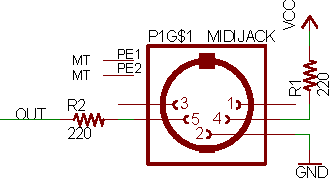
\includegraphics[keepaspectratio=true,width=0.6\columnwidth]{images/midi_out.pdf}
	\caption{MIDI output circuit, UART sends \emph{OUT} signal}
	\label{fig:midi_out}
\end{figurehere}

\begin{figurehere}
	\centering
	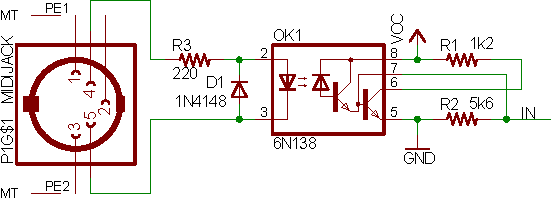
\includegraphics[keepaspectratio=true,width=\columnwidth]{images/midi_in.pdf}
	\caption{MIDI input circuit, UART receives \emph{IN} signal}
	\label{fig:midi_in}
\end{figurehere}


\paragraph{Basic protocol}
The serial protocol is 8-bits per message word, with one start (low) and one
stop (high) bits, MSb first, 31250 baud. The protocol is message-driven, with
standard messages 3 bytes long. Special messages are 1 to 3 bytes long, while
manufacturer-defined \emph{System Exclusive} (\emph{SysEx}) messages can be
arbitrarily long. Most of the messages were associated to common synthesizer
features \cite{midi_messages}, even tough manufacturers often interpret them
freely (e.g. through \emph{remapping}).

The first word of a message (control word) is always identified by the MSb
set to 1, while it is always 0 for data words, which are always 7 bits wide.

Standard messages are those referred to the actual music content, such as
\emph{Note On/Off}, \emph{Control Change}, \emph{Pitch Change} and so on,
also called \emph{voice messages}. A timing diagram of a voice message is
shown in \citef{fig:midi_voice_msg}.

The control word identifies the message type and the channel number. The
second word is usually the identifier of the control (key, knob, slider,
wheel, etc.) being actioned, and the third word tells its value or velocity.

Special messages include transport control (time, position), program selection,
system messages, etc. These are advanced messages, often only partially
supported, if not at all, by cheap controllers.

\begin{figure*}[t]
	\centering
	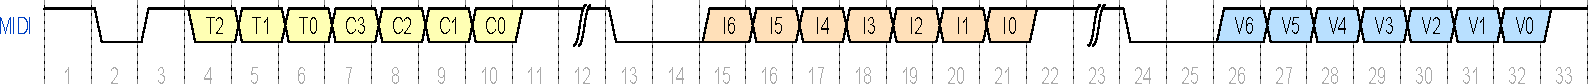
\includegraphics[keepaspectratio=true,width=\textwidth]{images/midi_voice_msg.pdf}
	\caption{Timing diagram of a MIDI voice message}
	\label{fig:midi_voice_msg}
\end{figure*}


\paragraph{Pros}
\begin{itemize*}
	\item \emph{De-facto} standard for digital music equipment
	\item Intuitive message semantics
	\item Simple, robust, noise-free, cheap hardware
\end{itemize*}


\paragraph{Cons}
\begin{itemize*}
	\item Slow communication
	\item No flow control
	\item Low resolution controls
	\item No streaming state support
\end{itemize*}


%-----------------------------------------------------------------------------
\subsection{MIDI/USB}

The \emph{Universal Serial Bus} (\emph{USB}) \cite{usb_docs} is probabily the
most available for consumer electronics interfacing nowadays. Its multipurpose
nature, speed, and robustness, made it the \emph{de-facto} standard for
connecting an actual \emph{universe} of devices. Among this huge load of
devices, also the digital music related ones can be found.

Since the MIDI standard was the most common digital music standard at the time
USB was released, it was convenient to encapsulate it inside USB packets.
So, an \emph{application protocol} was developed over the USB protocol: the
\emph{MIDI over USB} (\emph{MIDI/USB}).

This way, compatibility with standard MIDI interfaces was kept. Production
software and hardware devices kept using it, an so did music production
people. USB is simply the low-level interface, which can be found on all
consumer computers.

MIDI/USB has some advantages over the plain MIDI protocol. Since USB has a
higher baud rate than MIDI, it is possible to reduce delays when handling
many messages in a short interval.

Also, MIDI/USB introduces the concept of \emph{cable}. It supports up to 16
cables, which are 16 virtual plain MIDI devices. This makes theoretically
possible to drive up to 16 hardware synthesizers through a single USB cable,
by displatching the 16 virtual cables to as many real plain MIDI devices.

The MIDI/USB protocol exploits the features of \emph{bulk} transfers. This
way, packets will not be lost, thanks to the flow control of USB bulk
transfers.

USB devices can also show many indipendent behaviors, by choosing different
application protocols per each USB endpoint. For example, this allows to have
a MIDI/USB device with an integrated HID/USB trackpad,
by using a single USB cable, like the \emph{Torq Xponent} \cite{maudio_xponent}.

All the MIDI drawbacks are kept, except for the baud rate and flow control.
The USB, by its time-shared nature, always introduces some delays -- at
least 1~ms per query, and a few milliseconds for software stack processing.
As a drawback of bulk transfers, the delivering time is uncertain, because
many retansmissions can be issued, or there is not enough free bandwidth on
the bus, introducing even more delay.


\paragraph{Basic protocol}
The MIDI/USB protocol is a \emph{sub-class} of the \emph{Audio class}, defined
by the USB standard \CITEME. This parent class is oriented to audio equipment
communication and control -- speakers, microphones, keyboards, controllers,
synthesizers, DSPs can all be driven by this class.

The packet is composed by a \emph{header byte}, and the remaining 3 bytes are
the encapsulated MIDI packet -- all but the SysEx messages, which have variable
length. The header byte indexes the cable, and defines the following MIDI
message type -- some bytes can be unused, and thus ignored by the USB parser.
SysEx messages are simply split into 3-bytes chunks, merged by the USB parser
when the trailing byte(s) are received.

The protocol supports \emph{bulk} USB transfers. They add flow control to bare
USB streams, which in order adds flow control to the encapsulated MIDI stream.
Bulk packets have the lowest priority over the USB bus, which could introduce
delays when the bus is saturated by \emph{interrupt} and \emph{isochronous}
endpoint transfers. Also, packet handshaking and retransmission may add
some delay too.


\paragraph{Pros}
\begin{itemize*}
	\item USB is \emph{de-facto} standard for consumer electronics
	\item Much higher bandwidth than plain MIDI
	\item Up to 16 virtual cables
	\item Multi-purpose device through a single USB cable
\end{itemize*}


\paragraph{Cons}
\begin{itemize*}
	\item All the MIDI drawbacks, except for baud rate and flow control
	\item Delays introduced by USB time-sharing and bulk transfers
\end{itemize*}


%-----------------------------------------------------------------------------
\subsection{HID/USB}

Besides MIDI/USB, another application protocol was developed to handle those
devices which interface with human beings, and is much widely implemented.
The \emph{Human Interface Device} (\emph{HID}), in fact, is an USB class
with huge flexibility and support -- it can be found in almost any USB device
with keys, knobs, sliders, simple displays, LEDs, control wheels and so on.

The flexibility of HID is justified by the way its sub-protocol is developed.
HID messages, called \emph{reports}, have a fixed structure, defined at the
moment the HID configuration of the device is sent to the host.

\TODO


\paragraph{Basic protocol}
\TODO


\paragraph{Pros}
\begin{itemize*}
	\item Highest USB priority
	\item State streaming
	\item \TODO
\end{itemize*}


\paragraph{Cons}
\begin{itemize*}
	\item Sill some USB delays
	\item Custom HID reports to parse
	\item \TODO
\end{itemize*}


%%%%%%%%%%%%%%%%%%%%%%%%%%%%%%%%%%%%%%%%%%%%%%%%%%%%%%%%%%%%%%%%%%%%%%%%%%%%%
\section*{Conclusions}
\label{Conclusions}

\TODO


%%%%%%%%%%%%%%%%%%%%%%%%%%%%%%%%%%%%%%%%%%%%%%%%%%%%%%%%%%%%%%%%%%%%%%%%%%%%%

% We suggest the use of JabRef for editing your bibliography file (Report.bib)
\bibliographystyle{splncs}
\bibliography{Report}

\end{multicols}
\end{document}
